% !TeX encoding = UTF-8
% 主文件--main.tex
\documentclass[
	type = bachelor,	% bachelor | master | doctor
	%submit,
	%openany,			% openany  | openright(default)
	fontset = windows,  % fandol   | windows  (normal)
]{cqutthesis}

% 在这个文件里载入其他对写作有帮助的宏包,或自定义命令等
\usepackage{mycfg}

\cqutsetup{
	% 论文的中文标题
	ChineseTitle		= {\ce{SO2}吸收填料塔设计},
	% 封面上的标题。总字数不要超过 36 个汉字长度。
	% 本科:可以一行或分两行写,如无第二行将 ChineseTitleLineB 留空或注释掉;
	% 封面标题首行
	ChineseTitleLineA	= {化工原理课程设计(论文)},
	% 封面标题次行
	ChineseTitleLineB	= {\ce{SO2}吸收填料塔设计},
	% 论文的英文标题,一般需要大写
	EnglishTitle		= {DESIGN OF \ce{SO2} ABSORPTION PACKED TOWER},
	% 作者的中文姓名
	author				= {刘抗非},
	% 班级(仅本科)
	class				= {化学工程与工艺三班},
	% 学号
	studentid			= {12115990136},
	% 学院(仅本科)
	school				= {化学化工学院},
	% 专业名称(仅本科)
	major				= {化学工程与工艺},
	% 导师的姓名与职称(仅本科)
	supervisor			= {李新利},
	% 专业负责人姓名(仅本科)
	msupervisor			= {郝江瑜},
	% 中文、英文关键词,各关键词间以西文逗号“,”分隔
	ChineseKeywords		= {\ce{SO2}吸收, 填料塔, 聚丙烯鲍尔环, 设计优化, 吸收效率},
	EnglishKeywords		= {\ce{SO2} absorption, packed tower, polypropylene Pall rings, design optimization, absorption efficiency},
	% 日期,请注意:务必使用形如“YYYY-MM-DD”的格式
	date				= {2024-09-10},
}

\begin{document}
	
	% 不显示页码
	\thispagestyle{empty}
	
	% 论文封面
	\begin{figure}[htbp]
		\centering
		
\includegraphics[height=1.5\textwidth, keepaspectratio]{cover.pdf}
	\end{figure}

	% 从此以大写罗马数字编页码
	\frontmatter
	
	% 任务书
	%% 任务书
\begin{taskbook}
	\taskinfo		% or use `\taskinfo*' for less lines.
	
	
	
	%%%  1.设计(论文)的主要任务及目标
	\taskitem
	
	按不同学号给定的任务参数如下表:
	
	\begin{table}[H]
		\centering
		\caption*{按不同学号给定的吸收填料塔参数表}
		\begin{tabular}{|c|c|c|c|c|}
			\hline
			\ce{SO2}吸收率 & \multicolumn{3}{c|}{混合气体处理量 (m³/h)} & 操作条件 \\
			\hline
			& 900 m³/h & 1000 m³/h & 1100 m³/h & \\
			\hline
			96 \% & 4-6 & 25-27 & 16-18 & 常压 \\
			\hline
			98 \% & 19-21 & 1-3 & 34-36 & 绝压120kPa \\
			\hline
			96 \% & 10-12 & 31-33 & 7-9 & 常压 \\
			\hline
			98 \% & 28-30 & 13-15 & 22-24 & 绝压120kPa \\
			\hline
			& 5.5\% & 6\% & 6.5\% & \\
			\hline
			& \multicolumn{3}{c|}{进塔气体中\ce{SO2}的摩尔分数} &  \\
			\hline
		\end{tabular}
	\end{table}
	
	依据学号查得个人任务如下:
	
	\textbf{设计一个\ce{SO2}吸收填料塔,在常温,绝压$\mathbf{120kPa}$操作条件下,处理气体流量为$\mathbf{1000m³/h}$,\ce{SO2}含量为$\mathbf{6.0\%}$的废气,要求\ce{SO2}吸收率大于等于$\mathbf{98\%}$,使用聚丙烯散装鲍尔环作为填料。}



	%%% 2.设计(论文)的基本要求和内容
	\taskitem
	1. 选择合适的填料规格;
	2. 计算所需填料塔的尺寸和高度;
	3. 确定吸收液(\ce{H2O})的循环量;
	4. 分析操作条件对吸收效率的影响;
	5. 提供详细的设计图纸和流程图;
	6. 编写设计说明书,包含计算过程和结果分析。
	\clearpage



	%%% 3.主要参考文献
	\taskitem
	\begin{bibenumerate}
		\item 刘海洋. \LaTeX\ 入门\cite{latexrumen} [M]. 北京 : 电子工业出版社, 2013.
		\item MITTELBACH F, GOOSSENS M, BRAAMS J, et al. The \LaTeX\ Companion[M]. 2nd ed. Reading, Massachusetts : Addison-Wesley, 2004.
	\end{bibenumerate}
	
	
	
	%%% 4.进度安排
	\taskitem
	\begin{table}[H]
		\centering
		\begin{tabularx}{.95\textwidth}{p{1.5em}|X|p{6em}}
			\hline
			& 设计(论文)各阶段名称 &	起止日期\\
			\hline
			1 & 文献调研与方案设计 &	2024-09-07 至 2024-09-08\\
			\hline
			2	& 填料塔尺寸计算 &	2024-09-09 至 2024-09-11\\
			\hline
			3 & 设计图纸绘制与说明书编写 & 2024-09-12 至 2024-09-20\\
			\hline
		\end{tabularx}
	\end{table}	
\end{taskbook}
	
	% 摘要
	%% 摘要
\begin{cabstract}
	本设计旨在开发一个处理量为$\mathbf{1000m³/h}$的\ce{SO2}吸收填料塔,进料气体中\ce{SO2}含量为$\mathbf{6.0\%}$,其余为空气。在常温、绝压$\mathbf{120kPa}$操作条件下,要求\ce{SO2}吸收率达到$\mathbf{98\%}$以上。设计中选用聚丙烯散装鲍尔环作为填料。通过计算填料塔的尺寸和高度,选择合适的填料类型和规格,确定吸收液的循环量和浓度,分析操作条件对吸收效率的影响,并提供详细的设计图纸和流程图。本项目的创新点包括:1. 采用高效填料提高吸收效率;2. 优化填料塔设计以减少能耗;3. 提供详细的设计说明书,包含计算过程和结果分析。
\end{cabstract}
	
	% 生成主目录
	\tableofcontents
	
	% 设计图纸目录,这与主目录独立
	% \listofdesignfigures
	
	% 前言 or 引言
	\begin{foreword}
	
	二氧化硫(\ce{SO2})作为一种主要的大气污染物,不仅会导致酸雨的形成,还会对人体健康造成严重危害,诱发呼吸系统疾病、视觉系统疾病等。如今,随着工业化进程的不断加快,\ce{SO2}排放量逐年递增,控制和治理二氧化硫成为环境保护和可持续发展的重要课题。
	
	在化工领域中处理废气的方式多种多样,吸收是多种方式中行之有效的一种,其基本思想是利用混合气体各组分在液体溶剂中溶解度的不同来达到分离混合气体各组分的目的。如何高效地利用吸收操作去除工业废气中的\ce{SO2},是亟待解决的问题之一。
	
	一般来说,完整的吸收过程应包括吸收和解吸两部分。在化工生产过程中,原料气的净化、气体产品的精制、治理有害气体、保护环境等方面都要用到吸收将气体混合物中的各个组分加以分离,其目的是:①回收或捕获气体混合物中的有用物质,以制取有价值的产品;②除去混合气体中的有害成分,使气体净化,以便进一步加工处理;或除去工业放空尾气中的有害物质,以免污染大气。
	
	考虑到\ce{SO2}具有腐蚀性,若采用板式塔结构\ce{SO2}会对塔板造成严重的腐蚀影响吸收塔的正常工作,故此次设计应选择填料塔设计。此外,填料塔结构简单、操作弹性大、压降较低、能耗较小、传质效率高、分离效率高,更适合大规模工业应用,治理废气。
	
	二氧化硫吸收填料塔,以水为溶剂,经济合理,净化度高,污染小。由于水和二氧化硫反应生成硫酸,同时也具有相当的利用价值。
	
\end{foreword}
	
	% 从此以阿拉伯数字编页码
	\mainmatter
	
	% 流程说明
	%%% 第一章
\chapter{吸收塔填料塔的设计方案}



%%% ===============================================
\section{吸收流程的选择}

工业上使用的吸收流程多种多样,可以从不同的角度进行分类。根据所用的吸收剂种类,有仅用一种吸收剂的一步吸收流程和使用两种吸收剂的两步吸收流程;根据所用塔设备数量,可分为单塔吸收流程和多塔吸收流程;根据塔内气液两相的流向,可分为逆流吸收流程、并流吸收流程等基本流程。此外,还有用于特定条件下的部分溶剂循环流程。吸收用塔设备要求使用较小直径的塔设备完成规定的处理量,塔板或填料层阻力小,具有良好的传质性能,操作弹性大,结构简单,造价低,便于安装、操作和维修等。

吸收过程一般具有液气比大的特点,因此更适用填料塔。其优点是阻力小,效率高,有利于过程节能。因此,对于吸收过程来说,填料塔应用较为广泛。填料塔的工艺设计内容是在明确了装置的处理量、操作温度及操作压力及相应的相平衡关系的条件下,完成填料塔工艺尺寸、其他塔内件设计及其他塔外件设计。

\subsection{单剂和多剂的选择}

一般来说,对于组分较为简单、分离要求不是很高的情况,可以优先考虑单剂吸收。而对于需要去除多种杂质或要求较高纯度的情况,则可能需要采用多剂吸收。在实际工程中,需要根据具体情况进行技术经济比较后做出选择。


\subsection{单塔和多塔的选择}

单塔吸收流程是吸收过程中最常用的流程,如过程无特别需要,则一般采用单塔吸收流程。若过程的分离要求较高,使用单塔操作时,所需要的塔体过高,或采用两步吸收流程时,则需要采用多塔流程(通常是双塔吸收流程)。

\subsection{逆流与并流的选择}

吸收塔或再生塔内气液相可以逆流操作也可以并流操作。由于逆流操作具有传质推动力大,分离效率高(具有多个理论级的分离能力)的显著优点而广泛应用。工程上,如无特别需要,一般均采用逆流吸收流程。本设计采用单塔逆流操作。



%%% ===============================================
\section{塔内填料的选择}

\textbf{散堆填料简述}:目前散堆填料主要有环形填料、鞍形填料、环鞍形填料及球形填料。所用的材质有陶瓷、塑料、石墨、玻璃及金属等。

\begin{enumerate}
	\item \textbf{拉西环填料}:拉西环填料于1914年由拉西(F. Rashching)发明,为外径与高度相等的圆环。拉西环填料的气液分布较差,传质效率低,阻力大,通量小,目前工业上已较少应用。
	
	\item \textbf{鲍尔环填料}:鲍尔环是对拉西环的改进,在拉西环的侧壁上开出两排长方形的窗孔,被切开的环壁的一侧仍与壁面相连,另一侧向环内弯曲,形成内伸的舌叶。鲍尔环由于环壁开孔,大大提高了环内空间及环内表面的利用率,气流阻力小,液体分布均匀。与拉西环相比,鲍尔环的气体通量可增加$50\%$以上,传质效率提高$30\%$左右,是一种应用较广的填料。
	
	\item \textbf{阶梯环填料}:阶梯环结构与鲍尔环填料相似,环壁上开有长方形小孔,环内有两层交错$45^{\circ}$的十字形叶片,环的一端成喇叭口形状的翻边。这样的结构使得阶梯环填料的性能在鲍尔环的基础上又有提高,其生产能力可提高约$10\%$,压降则可降低$25\%$。阶梯环一般由塑料和金属制成,性能优于其他侧壁上开孔的填料,应用广泛。
	\item \textbf{矩鞍填料}:矩鞍填料堆积时不会套叠,液体分布较均匀。一般采用瓷质材料制成,其性能优于拉西环。目前,国内绝大多数应用瓷拉西环的场合,均已被瓷矩鞍填料所取代。
	
	\item \textbf{金属环矩鞍填料}:环矩鞍填料兼顾环形和鞍形结构特点而设计出的一种新型填料,一般以金属材质制成,故又称为金属环矩鞍填料。其综合性能优于鲍尔环和阶梯环,在散装填料中应用较多。
\end{enumerate}

\textbf{填料性能的优劣}:通常根据效率、通量及压降三要素衡量。在相同的操作条件下,填料的比表面积越大,气液分布越均匀,表面的润湿性能越好,则传质效率越高;填料的空隙率越大,结构越开敞,则通量越大,压降亦越低。按上述选择标准,同时考虑任务书要求,本设计将使用聚丙烯散装鲍尔环作为填料。选用聚丙烯材质的鲍尔环具有以下优点:
\begin{enumerate}
	\item \textbf{耐腐蚀性}:适用于\ce{SO2}吸收过程中的酸性环境;
	
	\item \textbf{质量较轻}:便于安装和更换;
	
	\item \textbf{成本较低}:有利于节省资金;
	
	\item \textbf{表面光滑}:有利于液体分布。
\end{enumerate}

\textbf{填料的规格的选择}:工业上工业塔常用散装填料主要有DN16、DN25、DN38、DN50、DN76 等规格。同类填料,尺寸越小,分离效率越高,但阻力增加,通量减小,填料费用也增加很多,因此,需要在分离效率和操作压力降之间找到合适的平衡点。而大尺寸的填料应用于小直径塔中,又会产生液体分布不良及严重的壁流,使塔的分离效率降低。应选择能够减少放大效应的填料,以保证塔内气液两相的均匀分布,选择结构易于拆装和清洁的填料,以减少维护成本和停机时间。

填料采用散装(乱堆)形式,因为散装形式能使气液相对充分接触,而且填料时省时省工。这种方式有利于提高传质效率,同时也简化了安装过程。

参考化工设备机械基础(第二版)413页,填料公称直径与塔的公称直径的关系,选择DN25聚丙烯散装鲍尔环。查化工原理课程设计148页表6-4可得$Φ_{F}=550 m^{-1} $,则根据表格选定,填料直径$d=25\,mm$,比表面积$a_{t}=175 m^{2}/m^{3}$, $\phi_{F}=550 \, m^{-1}$

\begin{table}[htbp] % 创建表格环境
	\centering % 居中
	\caption{聚丙烯散装鲍尔环参数表} % 添加表格标题
	\begin{tabular}{|c|c|c|c|c|c|}
		\hline 
		\multicolumn{3}{|l|}{产品名称} & \multicolumn{3}{|l|}{塑料鲍尔环} \\
		\hline 
		\multicolumn{3}{|l|}{材质} & \multicolumn{3}{|l|}{$PP/RPP/PVC/CPVC/PVDF/PTFE, PTFE$} \\
		\hline 
		\multicolumn{3}{|l|}{使用寿命} & \multicolumn{3}{|l|}{$>3 \, years$} \\
		\hline 
		\begin{tabular}{l}
			尺寸 \\
			$(mm)$
		\end{tabular} 
		& \begin{tabular}{l} 
			比表面积 \\
			$(m^2/m^3)$
		\end{tabular} 
		& \begin{tabular}{l} 
			空隙率 \\
			$(\%)$
		\end{tabular} 
		& \begin{tabular}{l} 
			堆积个数 \\
			$(\text{pieces/}m^3)$
		\end{tabular} 
		& \begin{tabular}{l} 
			堆积重量 \\
			$(kg/m^3)$
		\end{tabular} 
		& \begin{tabular}{l} 
			干填料因子 \\
			$(m^{-1})$
		\end{tabular} \\
		\hline 
		$16  \times 16  \times 1.0$ & $188$  & $91$ & $170000$ & $85$ & $275$ \\
		\hline 
		$25  \times 25  \times 1.2$ & $175$  & $90$ & $53500$  & $69$ & $239$ \\
		\hline 
		$38  \times 38  \times 1.4$ & $115$  & $89$ & $15800$  & $69$ & $220$ \\
		\hline 
		$50  \times 50  \times 1.5$ & $93 $  & $90$ & $6500$   & $52$ & $127$ \\
		\hline 
		$76  \times 76  \times 2.6$ & $73.2$ & $92$ & $1927$   & $48$ & $94$ \\
		\hline 
		$100 \times 100 \times 3.0$ & $52.8$ & $94$ & $1000$   & $48$ & $82$ \\
		\hline
	\end{tabular}
\end{table}



%%% ===============================================
\section{吸收剂的选择}

吸收剂的性能对吸收操作效果至关重要。选择吸收剂时应重点考虑以下几个方面:

\begin{enumerate}
	\item \textbf{溶解度}: 吸收剂对溶质组分的溶解度应大,以提高吸收速率并减少吸收剂用量。
	
	\item \textbf{选择性}: 吸收剂应对目标溶质组分有良好的吸收能力,而对混合气体中的其他组分不吸收或吸收甚微,以实现有效分离。
	
	\item \textbf{挥发度}: 在操作温度下,吸收剂的蒸气压应低,以减少吸收和再生过程中的吸收剂挥发损失。
	
	\item \textbf{粘度}: 在操作温度下,吸收剂的粘度越低越好,这有助于提高其在塔内的流动性,进而提高传质速率和传热速率。
	
	\item \textbf{其他性质}: 理想的吸收剂还应尽可能满足以下要求:无毒性、无腐蚀性、不易燃易爆、不发泡、冰点低、价格低廉,易于获得、化学性质稳定
\end{enumerate}

由于在常温$20^{\circ}$C下,操作压力(绝压,下同)为$120kPa$下,水对\ce{SO2}有较大的溶解度, 有较好的化学稳定性, 有较低的黏度, 且廉价、易得、无毒、不易燃烧, 所以可选择$20^{\circ}$C清水作为吸收剂。



%%% ===============================================
\section{操作条件的选择}

\begin{enumerate}
	\item \textbf{操作温度的确定}: 由吸收过程的气液平衡关系可知,对于物理吸收过程,较低的操作温度有利于提高溶质的溶解度,但过低温度可能会增加操作费用和能耗。同时较高的操作温度虽然会加快化学反应的速率,但也会降低传质推动力。
	
	\item \textbf{操作压力的确定}: 由吸收过程的汽液平衡关系可知,提高操作压力可以提高气体在液体中的溶解度,增加吸收的推动力。但随着操作压力的升高,对设备的加工制造要求提高,且能耗增加,因此需结合具体工艺条件综合考虑,以确定操作压力。
\end{enumerate}

由此,在本次\ce{SO2}吸收设计中,操作温度为常温即设定为$20^{\circ}$C,操作压力为$120kPa$。



\clearpage
%%% ===============================================
\section{工艺流程图}

\begin{figure}[h]
	\centering
	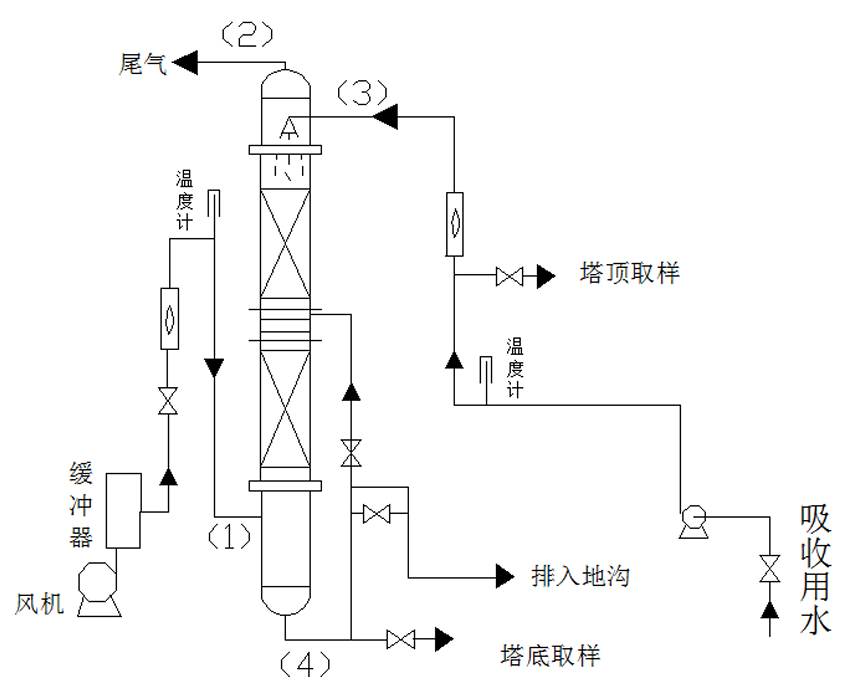
\includegraphics[width=0.8\textwidth]{./figure/吸收塔工艺流程示意图.png}
	\caption{吸收塔工艺流程示意图}
\end{figure}
	
	% 吸收塔工艺计算
	%%% 第二章
\chapter{吸收填料塔工艺参数计算}

在进行吸收填料塔工艺参数的设计\cite{Design-of-Packed-Absorption-Column}时,本章首先进行基础数据的准备,然后依据相应的逻辑流程图进行计算,校核,以确定过程中的具体参数,相关计算由计算机程序计算,程序代码见附录\ref{code:absorabsorption_column}。

%%% ===============================================
\section{基础物性数据}

\subsection{气相物性数据}

对于气相,重要的物性包括混合气体的平均摩尔质量、混合气体的平均密度和混合气体的黏度。而混合气体的黏度由于\ce{SO2}含量较低,混合气体黏度可以近似取为空气的黏度。已知\ce{SO2}的摩尔质量$M_{\ce{SO2}}$为$64.06 \, g/mol$,空气的摩尔质量$M_{Air}$为$28.95 \, g/mol$,理想气体常数$R=8.314 \, m^3 \cdot kPa/(kmol \cdot K)$,则所需数据按理想气体状态方程计算如下:

混合气体的平均摩尔质量:
\begin{equation}
	\overline{M_{V}} = 0.060 \times 64.06 + (1-0.060) \times 28.95 = 31.0566 \, g/mol
\end{equation}

混合气体的平均密度为:
\begin{equation}
	\rho_{V}=\frac{PM_{V}}{RT}=\frac{120\times31.0566}{8.314\times(273.15+20)}=1.4291 \, kg/m^3
\end{equation}

混合气体黏度可近似取为空气黏度。查化工原理上册教材附录338页,得20°C时空气的黏度:
\begin{equation}
	\mu_{V}	= \mu_{Air}=1.81\times10^{-5} \, Pa \cdot s = 0.060 \, kg/(m \cdot h)
\end{equation} 

查化工原理课程设计得20°C时\ce{SO2}在空气中的扩散系数:
\begin{equation}
	D_{V}=0.108 \, cm^2/s = 0.039 \, m^2/h
\end{equation}

\subsection{液相物性数据}

对于低浓度吸收过程,溶液的物性数据可近似取水的物性数据。重要的液相物性包括密度、黏度、表面张力和\ce{SO2}在水中的扩散系数。由化工原理实验教材127页水的重要物理性质表得20°C时水的有关物性数据如下:

水的密度:
\begin{equation}
	\rho_{L} = 998.2 \, kg/m^3
\end{equation}

水的黏度:
\begin{equation}
	\mu_{L} = 1.005 \, mPa \cdot s = 0.001005 Pa \cdot s = 3.618 \, kg/(m \cdot h)
\end{equation}

水的表面张力:
\begin{equation}
	\sigma_{L} = 7.28 \times 10^{-2} = 0.0728\, N/m
\end{equation}

\ce{SO2}在水中的扩散系数:
\begin{equation}
	D_{L} = 1.47 \times 10^{-9} \, m^2/s = 5.292 \times 10^{-6} \, m^2/h
\end{equation}

\subsection{气液相平衡数据}

在吸收塔设计中,气液相平衡数据是确定传质驱动力的关键。对于\ce{SO2}在水中的溶解,我们需要考虑亨利系数、相平衡常数和溶解度系数。查教材82页表2-1得,常压下20°C时\ce{SO2}在水中的相关数据如下:

亨利系数:
\begin{equation}
	E = 0.355 \times 10^{4} = 3.55 \times 10^{3} \, kPa
\end{equation}

相平衡常数:
\begin{equation}
	m = \frac{E}{P} = 29.5833
\end{equation}

溶解度系数:
\begin{equation}
	H = \frac{\rho_{L}}{EM_{\ce{SO2}}} = 0.0156039 \, kmol/(kPa \cdot m^3)
\end{equation}
其中,$P$为系统压力,$\rho_{L}$为液相密度,$M_{\ce{SO2}}$为\ce{SO2}的摩尔质量。



%%% ===============================================
\section{物料衡算}

根据设计要求得知,进口气体的体积流量 $V'=1000 \, m³/h$,二氧化硫的摩尔分数为 $y_1=0.060$,二氧化硫吸收率 $η=98\%$。

进塔气相摩尔比:
\begin{equation}
	Y_1 = \frac{y_1}{1-y_1} = 0.0638298
\end{equation}

出塔气相摩尔比:
\begin{equation}
	Y_2 = Y_1(1-η) = 0.0012766
\end{equation}

进塔惰性气相流量:
\begin{equation}
	V = \frac{V'}{22.4} \times (1-y_1) \times \frac{273}{273+20} = 39.0998 \: kmol/h
\end{equation}

该吸收过程属于低浓度吸收,平衡关系为直线,因此最小液气比为:
\begin{equation}
	\left(\frac{L}{V}\right)_{min} = \frac{Y_1 - Y_2}{Y_1/m - X_2} = 28.9917
\end{equation}
式中:$X_2=0$,$L$ 为液相流量,$V$ 为气相流量。

一般情况下,吸收剂用量为吸收剂最小用量的 $1.1 \sim 2.0$ 倍,这里取操作液气比为 $1.4$ 倍最小液气比。
\begin{equation}
	\frac{L}{V} = 1.4 \left(\frac{L}{V}\right)_{min} = 40.5883
\end{equation}

吸收剂用量:
\begin{equation}
	L = 40.5883 \times 39.0998 = 1587 \: kmol/h
\end{equation}

物料衡算:
\begin{equation}
	V(Y_1-Y_2) = L(X_1-X_2)
\end{equation}
得 $X_1 = 0.00154116$



%%% ===============================================
\section{填料塔工艺尺寸计算}

\subsection{填料塔塔径的计算}

采用 Eckert 通用关联图计算泛点气速。液相质量流量可近似按纯水流量计算,即液相质量流量为:
\begin{equation}
	W_{L} = 1587 \times 18.02 = 28597.7 \, kg/h
\end{equation}

气相质量流量为:
\begin{equation}
	W_{V} = 1000 \times 1.4291 = 1529.1 \, kg/h
\end{equation}

后续计算按逻辑流程图如下:
\begin{figure}[hbtp]
	\centering
	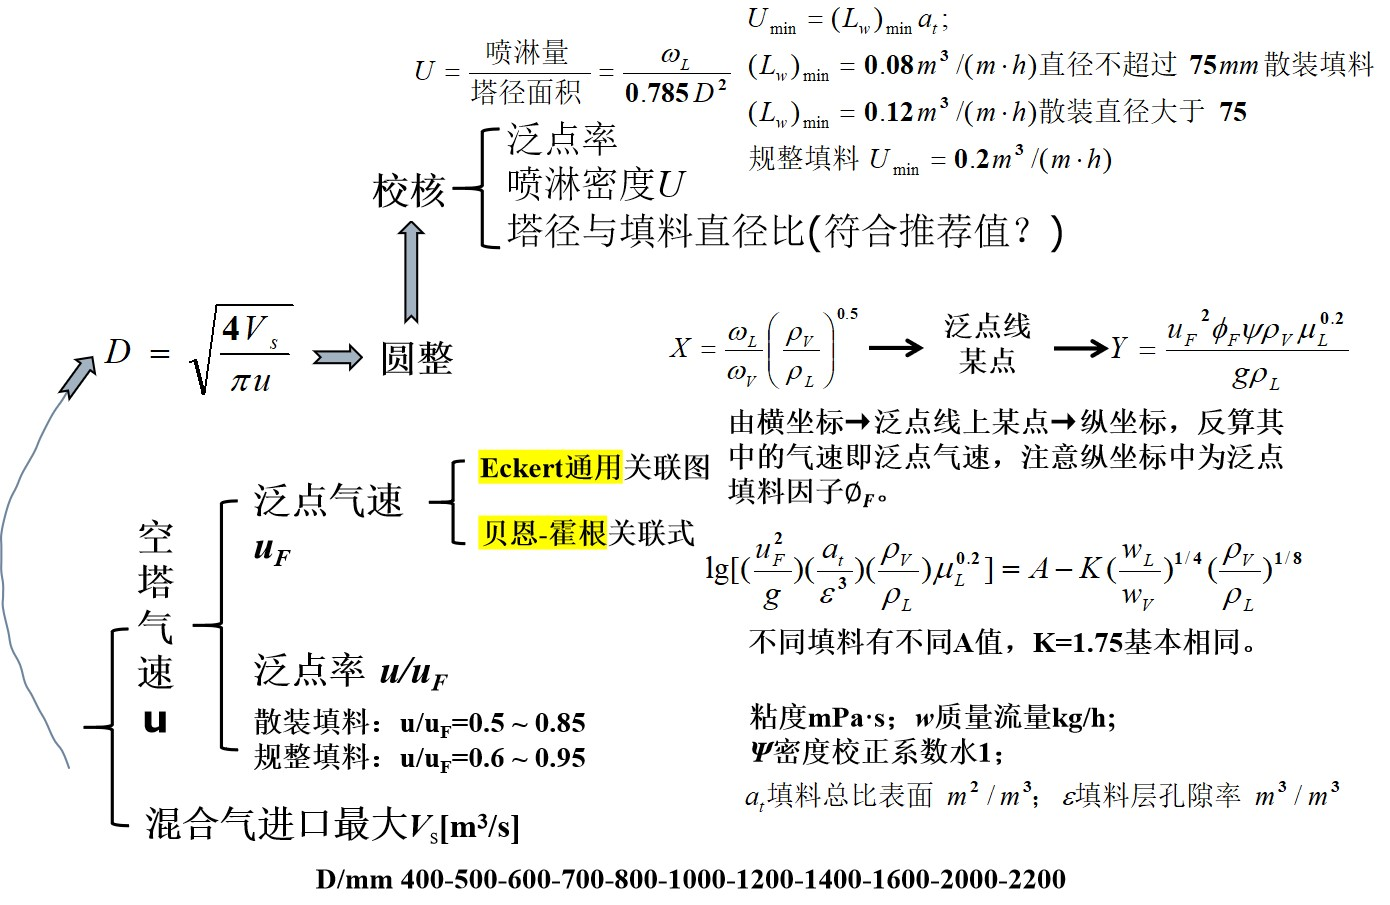
\includegraphics[width=0.80\textwidth]{塔径设计相关逻辑.jpg}
	\captionsetup{skip=2pt} % 内部定义的captionsetup,设置描述与图的间距
	\caption{泛点气速-塔径相关逻辑示意图}
	\label{fig:塔径计算相关逻辑流程图}
\end{figure}

Eckert 通用关联图的横纵坐标值分别为:
\begin{equation}
	X_{Eckert} = \frac{W_{L}}{W_{V}} \left( \frac{\rho_{V}}{\rho_{L}} \right)^{0.5} = 0.731989
\end{equation}

查 Eckert 通用关联图得:
\begin{equation}
	Y_{Eckert} = \frac{u_F^2 \phi \varphi \rho_{V}}{g \rho_{L} \mu_{L}^{0.2}} = 0.034
\end{equation}
式中:$u_F$ 为泛点气速,m/s;$\rho_{V}$ 为气相密度,kg/m³;$\rho_{L}$ 为液相密度,kg/m³;$\mu_{L}$ 为液体黏度,mPa·s;$\phi$ 为实验填料因子,$g$ 为重力加速度,9.81 m/s²;$\varphi$ 为水的密度与液体密度之比,此处为$1$。

由化工原理课程设计教材 148 页表 6-4 得 $\phi = 184 \, m^{-1}$,则:

\begin{equation}
	u_F = \sqrt{\frac{Y_{Eckert} g \rho_{L}}{\phi \varphi \rho_{V} \mu_{L}^{0.2}}} = \sqrt{\frac{0.034 g \rho_{L}}{\phi \varphi \rho_{V} \mu_{L}^{0.2}}} = 0.9 28879 \, m/s
\end{equation}

取 $u = 0.7 u_F = 0.440215 \, m/s$,有:

\begin{equation}
	D = \sqrt{\frac{4V_{s}}{\pi u}} = \sqrt{\frac{4 \times 1000/3900}{3.14 \times 0.440215}} = 0.896337 \, m = 896.337 \, mm
\end{equation}
圆整塔径,取$D=0.9 m$,也即$D=900mm$。

\subsection{填料塔塔径的校核}

\textbf{泛点率校核}:
泛点率是塔内实际操作气速与泛点气速的比值,一般要求在 50\% $\sim$ 80\%之间。
\begin{equation}
	u =(1000/3900)/(\frac{\pi}{4} \times 0.9 ^2)= 0.436639 m/s
\end{equation}
\begin{equation}
	u/u_{F} = 0.436639 / 0.9 28879 = 0.694313 \text{ (在允许范围 0.50-0.85 之内)}
\end{equation}

\textbf{填料规格校核}:

当塔径与填料外径之比(即径比)过小时,塔的性能会变得不稳定。因为径比过小时,靠近塔壁的填料层的空隙率会增大且不均匀,塔的通过能力虽然会有所提升,但由于气流短路,塔的效率反而会下降。所以需要对填料规格进行校核,以下是常用填料的径比下限。

\begin{table}[h]
	\centering
	\caption{填料种类及其推荐值} % 添加表格标题
	\begin{tabularx}{\textwidth}{|X|X|} % 控制表格宽度为文本宽度
		\hline 
		\textbf{填料种类} & \textbf{$D/d$ 推荐值} \\
		\hline 
		拉西环 & $D/d \geq 20 \sim 30$ \\
		\hline 
		鞍环 & $D/d \geq 15$ \\
		\hline 
		鲍尔环 & $D/d \geq 10 \sim 15$ \\
		\hline 
		阶梯环 & $D/d > 8$ \\ % 修改了这里的符号
		\hline 
		环矩鞍 & $D/d > 8$ \\
		\hline
	\end{tabularx}
\end{table}
进行校核有:
\begin{equation}
	D/ d = 900/ 38 = 23.6842 > 10
\end{equation}

\textbf{液体喷淋密度校核}:
最小润湿速率是指塔的截面上,单位长度的填料周边的最小液体流体体积。直径不超过 75 mm 的散装填料,最小润湿速率为:
\begin{equation}
	(L_{W})_{min}=0.08m^{3}/(m \cdot h)
\end{equation}

由化工原理教材 325 页的聚丙烯鲍尔环特性数据表得
\begin{equation}
	a_{t}=175 \, m^2/m^3
\end{equation}
\begin{equation}
	U_{\min}=(L_{W})_{\min}a_{t}=14m^{3}/(m^{2}\cdot h)
\end{equation}
\begin{equation}
	U=\frac{28597.7/998.2}{\frac{\pi}{4}\times0.9 ^2}=45.0338 m^3/(m^2\cdot h)>U_{min}
\end{equation}
故满足最小喷淋密度的要求。经以上校核可知,填料塔直径 $D=900 mm$ 合理。

\subsection{传质单元数的计算}

脱析因数 \( S \) 计算如下:
\begin{equation}
	S = \frac{mV}{L} = \frac{29.5833}{40.5883} = 0.728863
\end{equation}

气相总传质单元数 \( N_{OG} \) 的计算为:
\begin{align}
	N_{OG}
	&= \frac{1}{1-S} \ln \left[\left(1-S\right)\frac{Y_1 - Y_2^{*}}{Y_2 - Y_2^{*}} + S\right] \\
	&= \frac{1}{1-0.728863} \ln \left[\left(1-0.728863\right)\frac{0.0582-0}{0.002328-0}+0.728863\right] \notag \\
	&= 9.80781  \notag
\end{align}

\subsection{膜吸收系数的计算}

\begin{figure}[ht]
	\centering
	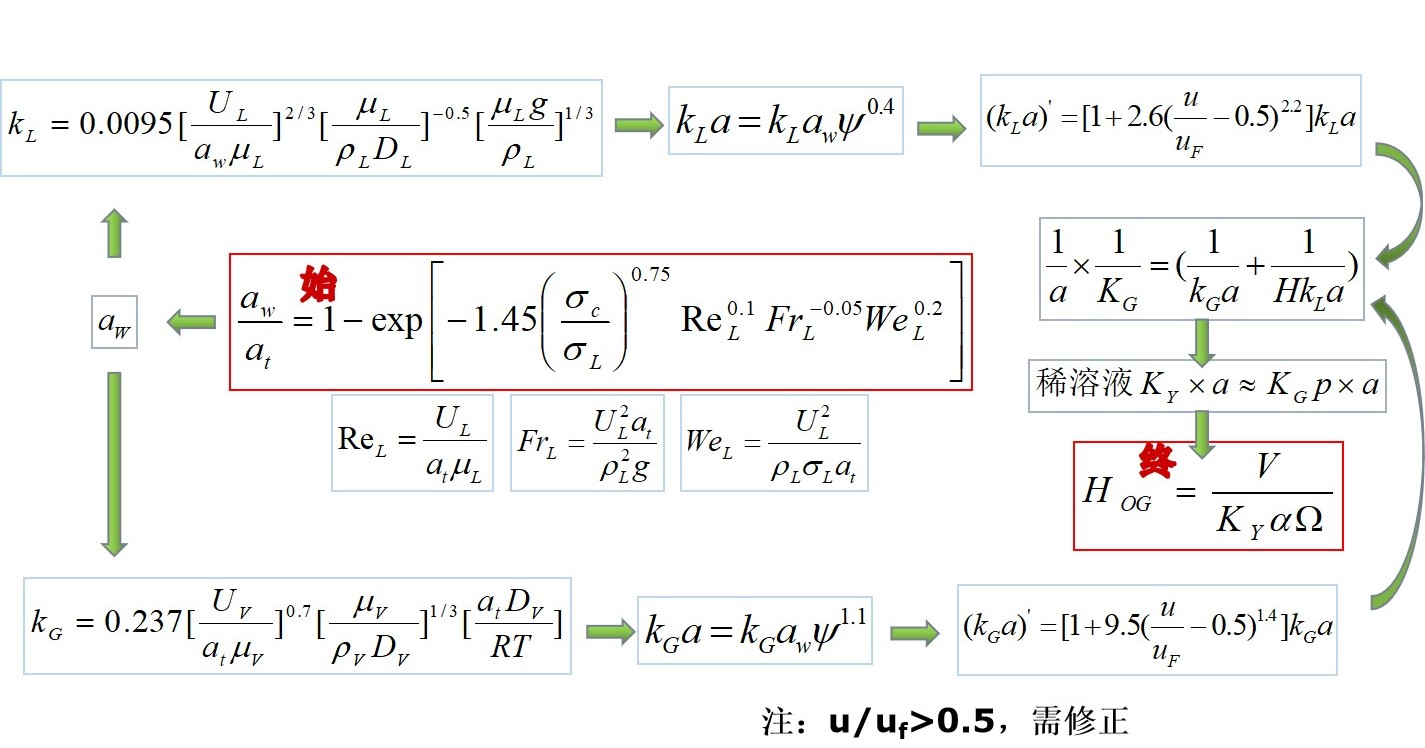
\includegraphics[width=0.8\textwidth]{传质单元高度.jpg}
	\caption{由膜吸收系数至传质单元高度的流程示意图}
\end{figure}

气相总传质单元高度采用修正的Onda关联式:
\begin{equation}
	\frac{a_{w}}{a_{t}} = 1-e^{-1.45\left(\frac{\sigma_c}{\sigma_w}\right)^{0.75}\left(\frac{U_{L}}{a_{t}\mu_{L}}\right)^{0.1}\left(\frac{U_{L}\mu_{L}}{\rho_{L}g}\right)^{-0.05}\left(\frac{U_{L}^2}{\rho_{L}\sigma_L a_{t}}\right)^{-0.2}}
\end{equation}

由化工原理课程设计教材中175页表6-6得$\sigma_{c} = 427680kg/h^{2}$

液体质量通量:
\begin{equation}
	U_{L} = \frac{28597.7}{\frac{\pi}{4} \times 0.9 ^2} = 44952.7 kg/(m^2·h)
\end{equation}

代入Onda关联式:
\begin{equation}
	\frac{a_{w}}{a_{t}} = 0.443873
\end{equation}

所以:
\begin{equation}
	a_{w} = 0.443873 \times 175 = 77.6778 \, m^2/m^3
\end{equation}

气体质量通量:
\begin{equation}
	U_{V} = \frac{1529.1}{\frac{\pi}{4} \times 0.9 ^2} = 2403.59 kg/(m^2·h)
\end{equation}

计算气侧吸收系数:
\begin{align}
	k_{G}
	&= 0.237\Bigg(\frac{U_{V}}{a_{t}\mu_{V}}\Bigg)^{0.7}\Bigg(\frac{\mu_{V}}{\rho_{V}D_{V}}\Bigg)^{1/3}\Bigg(\frac{a_{t}D_{V}}{RT}\Bigg) \\
	&=
	0.0288785 \, kmol/(m^2·h·kPa) \notag
\end{align}

计算液膜吸收系数:
\begin{align}
	k_{L}
	&= 0.0095\biggl(\frac{U_{L}}{a_{w}\mu_{L}}\biggr)^{2/3}\biggl(\frac{\mu_{L}}{\rho_{L}D_{L}}\biggr)^{-1/2}\biggl(\frac{\mu_{L}g}{\rho_{L}}\biggr)^{1/3} \\
	&=
	0.826184 \, m/h \notag
\end{align}

\subsection{总传质系数的计算}

\textbf{体积吸收系数}:

由化工原理课程设计教材175页表6-7得参数 $\psi = 1.45$,计算 $k_Ga$ 和 $k_La$ 如下:
\begin{align}
	k_{G}a
	&= k_{G}a_{W} \psi^{1.1} \\
	&= 0.0288785 \times 91.0681 \times 1.45^{1.1} \notag \\
	&= 3.3758 \, kmol/(m^3 \cdot h \cdot kPa) \notag
\end{align}
\begin{align}
	k_{L}a
	&= k_{L}a_{W} \psi^{0.4} \\
	&= 0.826184 \times 91.0681 \times 1.45^{0.4} \notag \\
	&= 74.4596 \, kmol/(m^3 \cdot h \cdot kPa) \notag
\end{align}

\textbf{修正体积吸收系数}:

由于 $u/u_F = 0.694313 > 0.5$,使用化工原理课程设计教材152页修正公式(6-12)与(6-13)进行修正:
\begin{align}
	k_{G}^{\prime}a
	&= \left[1 + 9.5 \left(\frac{u}{u_{F}} - 0.5\right)^{1.4}\right] k_{G}a \\
	&= 6.61176 \, kmol/(m^3 \cdot h \cdot kPa) \notag
\end{align}
\begin{align}
	k_{L}^{\prime}a
	&= \left[1 + 2.6 \left(\frac{u}{u_{F}} - 0.5\right)^{2.2}\right] k_{L}a \\
	&= 79.727 \, kmol/(m^3 \cdot h \cdot kPa) \notag
\end{align}

\textbf{总体积传质系数}:
\begin{equation}
	K_{G}a = \frac{1}{\frac{1}{k_{G}^{\prime}a} + \frac{1}{H k_{L}^{\prime}a}} = 1.04705 \, kmol/(m^3 \cdot h \cdot kPa)
\end{equation}

\subsection{填料层高度的计算}

计算填料层高度 $H_{OG}$ 和总高度 $Z$:
\begin{equation}
	H_{OG} = \frac{V}{K_{G}a p_{总} \Omega} = 0.489162 \, m
\end{equation}
\begin{equation}
	Z = H_{OG} \cdot N_{OG} = 4.79761 \, m
\end{equation}
\begin{equation}
	Z^{\prime} = 1.25Z = 5.99701 \, m
\end{equation}
设计取填料层高度为 $Z^{\prime} = 5.99701 \, m < h_{max} = 6 \, m$,故不进行分段。

\subsection{填料层压降的计算}
填料层压降直接影响到填料塔的能效和操作性能。压降的大小决定了塔内气体的流动状态,过高的压降会增加泵送能耗,降低塔的处理能力和操作灵活性。而过低的压降可能意味着填料层的传质效率不足,影响塔的分离效率。

在设计阶段,通过计算填料层压降,可以选择合适的填料类型和尺寸,以及确定塔的操作参数,确保塔在经济和技术上的可行性。在操作阶段,监控和调整填料层压降有助于维持塔内气液两相的理想流动状态,避免出现液泛等不稳定现象,从而保证塔的稳定运行和提高产品质量。 因此,填料层压降的计算是填料吸收塔设计和优化中的一个基本步骤,对于实现高效、节能和安全的化工生产具有重要意义。

\begin{figure}[ht]
	\centering
	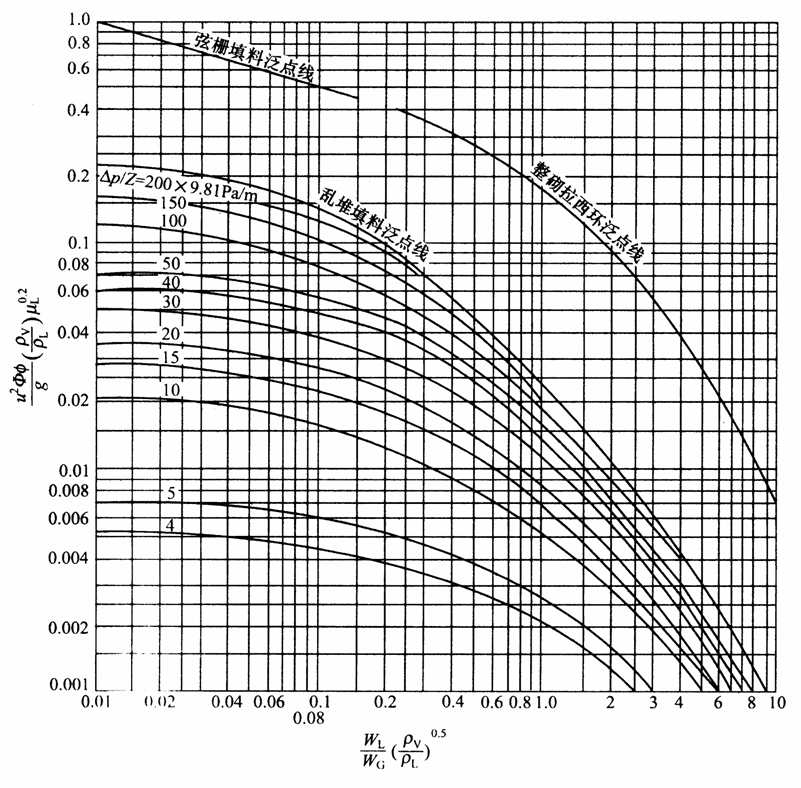
\includegraphics[width=0.6\textwidth]{Eckert关联图.png}
	\caption{Eckert通用关联图}
\end{figure}

采用埃克特通用关联图计算填料层压降,Eckert 通用关联图的横坐标值为:
\begin{equation}
	X_{Eckert} = \frac{W_{L}}{W_{V}} \left( \frac{\rho_{V}}{\rho_{L}} \right)^{0.5} = 0.731989
\end{equation}

查化工原理课程设计 154 页表 6-11可得$\phi_{p}=232m^{-1}$,则
纵坐标为:
\begin{equation}
	Y_{Eckert} = \frac{u_F^2 \phi_{p} \varphi \rho_{V}}{g \rho_{L} \mu_{L}^{0.2}} = 0.00893255
\end{equation}
式中:$u_F$ 为泛点气速,m/s;$\rho_{V}$ 为气相密度,kg/m³;$\rho_{L}$ 为液相密度,kg/m³;$\mu_{L}$ 为液体黏度,mPa·s;$\phi_{p}$ 为填料层压降的实验填料因子,$g$ 为重力加速度,9.81 m/s²;$\varphi$ 为水的密度与液体密度之比,此处为$1$。

查化工原理课程设计 148 页图 6-2,得单位填料层压降:
\begin{equation}
	\Delta p/Z = 9 \times 9.81 = 88.29 \, Pa/m
\end{equation}

则填料层压降:
\begin{equation}
	\Delta p=88.29\times5.7 \, Pa = 503.253 \, Pa
\end{equation}

\subsection{塔附属高度的计算}
塔的附属高度包括上部空间、液体分布器空间和底部空间。根据设计,塔的上部空间取1.0米,底部空间取1.1米,液体分布器高度为0.2米,因此塔的附属高度为:

\begin{equation}
	H_{\text{附属}} = 1.0 + 1.1 + 0.2 = 2.3 \, m
\end{equation}



%%% ===============================================
\section{吸收塔工艺尺寸总结}
吸收塔工艺计算的目的是确保设备能够在实际操作中高效、稳定地进行传质操作,并满足设计要求。通过严密的气液传质模型和物料衡算,我们能够设计出适合特定工艺条件的吸收塔。

首先,在物性数据的获取与应用中,通过对气液相物理性质如密度、黏度、扩散系数等的准确估算,保证了后续计算的可靠性。特别是亨利系数等气液相平衡数据的获取,为传质驱动力的计算提供了坚实的基础。

在物料衡算中,基于已知的气体流量、二氧化硫的浓度及吸收率,计算出进出塔的气相摩尔比、惰性气体流量及最小液气比,并确定了实际操作中的液气比。通过这些数据,可以进一步推导出吸收剂的用量,确保吸收操作能够实现高效的二氧化硫去除。

随后,在填料塔的尺寸设计中,利用Eckert通用关联图和相关实验参数,计算出泛点气速、塔径及填料层高度,并进行了校核。通过对泛点率、填料规格及液体喷淋密度的核查,确保塔的设计既能满足工艺需求,又不会出现气流短路或液泛等不良现象。此外,对填料层压降的计算也表明塔内流体流动阻力在合理范围内,保证了塔的能耗在可接受的范围。

在传质计算中,应用膜吸收系数、Onda关联式以及修正体积吸收系数,确保了传质效率的准确估计。通过计算气侧和液侧的传质单元数及传质单元高度,得出合适的填料层高度,保证气液传质能够在塔内有效进行。

最后,通过附属高度的设计,包括塔的上部空间、液体分布器及底部空间的合理布置,确保塔的整体结构稳定性和操作便利性。在附属设备的设计中,液体分布器和再分布器的合理配置,能够有效改善塔内流体的分布,减少局部液体聚集或气流短路的情况,从而进一步提高塔的效率。

总而言之,吸收塔的工艺计算不仅包括物料衡算、传质单元和填料层高度等核心内容,还涉及到结构设计、流体力学参数和操作稳定性的校核。通过这一系列精确的计算与校核,吸收塔的设计可以确保其在实际工业操作中具有高效的传质性能和良好的操作稳定性,从而实现高效的二氧化硫吸收和废气处理目标。

\clearpage

\begin{longtable}{
		@{} p{0.30\textwidth} p{0.20\textwidth} 
		p{0.20\textwidth} p{0.25\textwidth} @{}
		}
	\caption{参数汇总表} \\
	\toprule
	描述信息 & 参数符号 & 参数值 & 单位 \\
	\midrule
	\endfirsthead
	
	\toprule
	描述信息 & 参数符号 & 参数值 & 单位 \\
	\midrule
	\endhead
	
	\midrule
	\multicolumn{4}{r}{\textit{——接下页}} \\
	\endfoot
	
	\bottomrule
	\endlastfoot
	
	摩尔质量 & $M_V$ & $31.0566$ & $g/mol$ \\
	气体密度 & $\rho_V$ & $1.4291$ & $kg/m^{3}$ \\
	气体扩散系数 & $D_V$ & $1.08 \times 10^{-5}$ & $m^{2}/s$ \\
	气体粘度 & $\mu_V$ & $1.81 \times 10^{-5}$ & $Pa·s$ \\
	亨利常数 & $E$ & $3550$ & kPa \\
	气体分子质量比 & $m$ & $29.5833$ & - \\
	液体密度 & $\rho_L$ & $998.2$ & $kg/m^{3}$ \\
	液体粘度 & $\mu_L$ & $1.005 \times 10^{-3}$ & $Pa·s$ \\
	表面张力 & $\sigma_L$ & $0.0728$ & $N/m$ \\
	液体扩散系数 & $D_L$ & $1.47 \times 10^{-9}$ & $m^{2}/s$ \\
	溶解度系数 & $H$ & $0.0156039$ & $kmol/(kPa·m^{2}$) \\
	进料气体组分 & $Y_1$ & $0.0638298$ & - \\
	出料气体组分 & $Y_2$ & $0.0012766$ & - \\
	气体流量 & $V$ & $39.0998$ & $kmol/h$ \\
	液气比 & $\left(\frac{L}{V}\right)_{min}$ & $28.9917$ & - \\
	最小液气比 & $\left(\frac{L}{V}\right)_{min \quad ratio}$ & $1.4$ & - \\
	实际液气比 & $\frac{L}{V}$ & $40.5883$ & - \\
	液体流量 & $L$ & $1587$ & $kmol/h$ \\
	进料液体组分 & $X_1$ & $0.00154116$ & - \\
	液体质量流量 & $W_L$ & $28597.7$ & $kg/h$ \\
	气体质量流量 & $W_V$ & $1529.1$ & $kg/h$ \\
	泛点气速Eckert坐标X值 & $X_{Eckert, \phi_F}$ & $0.731989$ & - \\
	泛点气速Eckert坐标Y值 & $Y_{Eckert, \phi_F}$ & $0.034$ & - \\
	泛点气速 & $u_F$ & $0.9 28879$ & $m/s$ \\
	设计气速 & $u_{design}$ & $0.440215$ & $m/s$ \\
	未圆整塔径 & $D$ & $0.896337$ & $m$ \\
	圆整后塔径 & $D_{rounded}$ & $0.9$ & - \\
	实际操作气速 & $u_{actual}$ & $0.436639$ & $m/s$ \\
	泛点率 & $flooding \, ratio$ & $0.9 94313$ & - \\
	圆整后塔径与填料直径比 & $\frac{D_rounded}{d}$ & $23.6842$ & - \\
	最小喷淋密度 & $U_{min}$ & $14$ & $m^{3}/(m^{2}·h)$ \\
	实际喷淋密度 & $U$ & $45.0338$ & $m^{3}/(m^{2}·h)$ \\
	脱吸因数 & $S$ & $0.728863$ & $m^{2}$ \\
	气相总传质单元数 & $N_{OG}$ & $9.80781$ & - \\
	液相质量通量 & $U_L$ & $44952.7$ & $kg/(m^{2}·h)$ \\
	有效比表面积比 & $\frac{a_w}{a_t}$ & $0.443873$ & - \\
	有效比表面积 & $a_w$ & $77.6778$ & $m^{2}/m^{3}$ \\
	气相质量通量 & $U_V$ & $2403.59$ & $kg/(m^{2}·h)$ \\
	气膜吸收系数 & $k_G$ & $0.0288785$ & $kmol/(m^{2}·h·kPa)$ \\
	液膜吸收系数 & $k_L$ & $0.826184$ & $m/h$ \\
	气膜体积吸收系数 & $k_{G}a$ & $3.3758$ & $kmol/(m^{2}·h·kPa)$ \\
	液膜体积吸收系数 & $k_{L}a$ & $74.4596$ & $m/h$ \\
	修正后的气膜体积吸收系数 & $k'_{G}a$ & $6.61176$ & $kmol/(m^{2}·h·kPa)$ \\
	修正后的液膜体积吸收系数 & $k'_{L}a$ & $79.727$ & $m/h$ \\
	总传质系数 & $K_{G}a$ & $1.04705$ & $kmol/(m^{2}·h·kPa)$ \\
	填料层高度 & $H_{OG}$ & $0.489162$ & $m$ \\
	总高度 & $Z$ & $4.79761$ & $m$ \\
	设计高度 & $Z'$ & $5.99701$ & $m$ \\
	填料层压降Eckert坐标X值 & $X_{Eckert, \phi_P}$ & $0.731989$ & - \\
	填料层压降Eckert坐标Y值 & $Y_{Eckert, \phi_P}$ & $0.00893255$ & - 
\end{longtable}
	
	% 吸收塔内部附件选择
	%%% 第三章
\chapter{吸收塔内部附件的选择}
填料塔内件是填料塔的重要组成部分,它们的设计和选择对填料塔的性能有着直接的影响。填料塔内件的设计需要考虑多种因素,包括塔的直径、操作压力、处理的物料性质、填料的类型和特性等。设计时还需要确保内件能够提供足够的强度和刚度,以承受操作中的压力波动、机械震动和温度变化。此外,内件的设计应促进气液的均匀分布,以提高传质效率和塔的整体性能。



%%% ===============================================
\section{液体分布器的选择}
液体分布器是填料塔中的关键内件,它的主要作用是将液体均匀地分布在填料层的顶部,或者在塔内的某一高度上进行再分布。液体分布器的性能直接影响填料的传质效率和操作弹性。合理的液体分布可以减少填料塔内的放大效应和端效应,提高塔的整体效率,减少塔的尺寸和造价。

液体分布器的工作原理是通过其设计的结构,将进入塔内的液体以均匀的方式分配到填料层上,确保液体能够在填料表面形成均匀的膜状流动,从而实现有效的气液接触和传质。设计要求包括液体分布均匀、操作弹性大、结构紧凑、气体流通面积大、具备液体收集、分布及气体分布功能等。

液体分布器的类型多样,可以根据其流体动力特性、形状、液体离开的形式、分布的次数以及组合方式进行分类。例如,按分布器流体动力分有重力型和压力型,按形状分有管式、槽式、盘式等,按液体离开形式分有孔流型和溢流型。液体分布器的选择依据主要包括分布质量、操作弹性、处理量、气体阻力、对水平度等多个方面。

为了确保液体分布器的正常运行和填料塔的高效操作,需要定期检查分布器的工作状态,包括液体分布的均匀性和压降。在维护时,应注意检查是否存在堵塞或磨损,并及时进行清理或更换。优化建议可能包括调整液体分布器的设计以适应特定的操作条件,或者采用新型抗堵塞的设计来提高塔内的操作弹性和减少维护工作量。

槽式液体分布器具有较大的操作弹性和极好的抗污堵性,特别适合于大气液负荷,应用范围非常广泛。所以本次\ce{SO2}设计中选用槽式液体分布器。

\clearpage

\begin{figure}
	\caption{槽式液体分布器示意图}
	\centering
	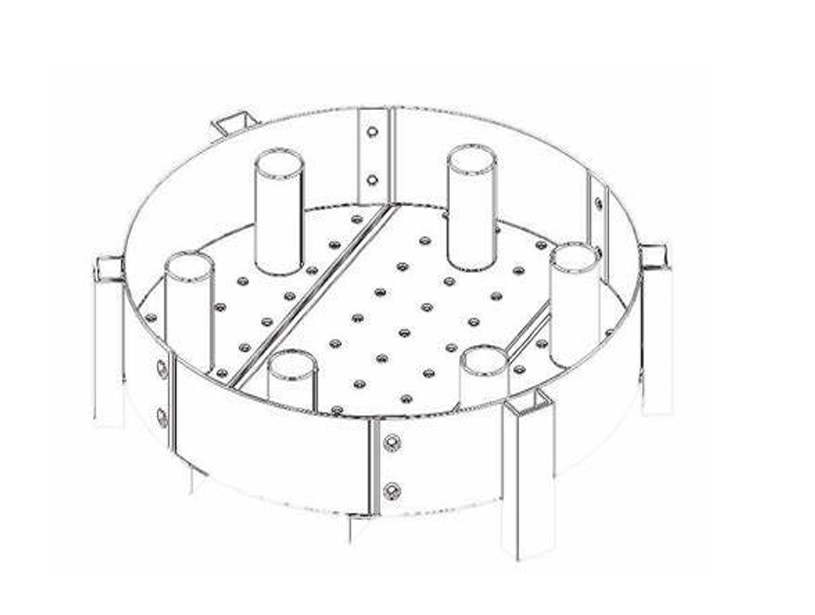
\includegraphics[width=\textwidth]{槽式液体分布器.png}
\end{figure}



%%% ===============================================
\section{液体再分布器的选择}
再分布器采用升气管式设计,适合大直径塔体。
除塔顶液体的分布之外,填料层中的液体的再分布是填料塔中的一个重要问题。往往会发现,在离填料顶面一定距离处,喷淋的液体便开始向塔壁偏流,然后雁塔壁下流,塔中心处填料得不到好的湿润,形成所谓“干椎体”的不正常现象,减少了气液两相的有效接触面积。因此每隔一定距离必须设置液体再分布器,以克服此种现象。升气管式再分布器适用于直径0.9 m以上的塔,而且可以分段卸下填料,更换填料方便,所以本设计选用升气管式再分布器



%%% ===============================================
\section{填料支承装置的选择}
填料支承装置的作用是支承填料以及填料层内液体的质量,同时保证气液两相顺利通过。支承若设计不当,填料塔的液泛可能首先发生在支承板上。为使气体能顺利通过,对于普通填料塔,支承件上的流体通过的自由截面积为填料面的50\%以上,且应大于填料的空隙率。此外,应考虑到装上填料后要将支承板上的截面堵去一些,所以设计时应取尽可能大的自由截面。自由截面太小,在操作中会产生拦液现象。增加压强降,降低效率,甚至形成液泛。由于填料支承装置本身对塔内气液的流动状态也会产生影响,因此作为填料支承装置,除考虑其对流体流动的影响外,一般情况下填料支承装置应满足如下要求:

足够的强度和刚度,以支持填料及所持液体的质量(持液量),并考虑填料空隙中的持液量,以及可能加于系统的压力波动,机械震动,温度波动等因素。

足够的开孔率(一般要大于填料的空隙率),以防止首先在支撑处发生液泛;为使气体能顺利通过,对于普通填料塔,支承件上的流体通过的自由截面积为填料面的50\%以上,且应大于填料的空隙率。此外,应考虑到装上填料后要将支承板上的截面堵去一些,所以设计时应取尽可能大的自由截面。自由截面太小,在操作中会产生拦液现象。增加压强降,降低效率,甚至形成液泛。

结构上应有利于气液相的均匀分布,同时不至于产生较大的阻力(一般阻力不大于20Pa)。本设计运用 的瓷质鲍尔环,孔隙率相对较大,升气管式支撑板能更好的克服支撑板的强度和自由截面之间的矛盾,耗能更好的适应高空隙率填料的要求,本设计选用升气管式支撑板。



%%% ===============================================
\section{填料压紧装置的选择}
填料支撑是填料塔内部的一个重要组成部分,它的主要作用是支撑填料层,确保填料在塔内均匀分布,防止填料在操作过程中发生下沉或移动,从而维持填料层的结构稳定性和传质效率。填料支撑还能够承受塔内的压力和机械负荷,保护塔体结构不受损害。

填料支撑的类型包括栅板式支撑、压板式支撑和驼峰支撑等。栅板式支撑通常由金属材料制成,具有一定的空隙率,可以放置在塔的支承圈上。压板式支撑则是制成栅板形状的填料压紧器,依靠自身重力将填料压紧。驼峰支撑则是通过冲压、切割等方式制成的立体结构,具有良好的力学性能和流体力学性能。

驼峰型支撑装置具有高刚性与载荷能力、优良流体分布性、节省材料,降低塔体重量,提升操作弹性和处理能力等优点。所以本次SO2吸收设计中选用驼峰型支撑装置。

压紧装置的作用是在填料塔操作过程中,通过施加压力来确保填料层的紧密性和稳定性。压紧装置通常安装在填料层的上方,可以是简单的重力式压紧,也可以是带有弹簧或其他机械装置的压紧系统。压紧装置的设计要能够适应不同操作条件下的压力变化,确保填料层在高压降或负荷波动时不会松动或破损。

为了确保填料支撑和压紧装置的正常运行,需要定期检查其结构的完整性和压紧效果。在维护时,应检查支撑结构是否有变形、腐蚀或损坏,并及时进行修复或更换。优化建议可能包括使用高质量的材料来提高支撑和压紧装置的耐久性,以及根据操作条件调整压紧力度,以达到最佳的传质效果和塔的运行效率。

填料压紧网板的设计要求有足够的空隙率,通常大于70\%,可以减少流体阻力并促进气液的均匀分布和防止填料从间隙中漏出。所以本次SO2吸收设计采用填料压紧网板。



%%% ===============================================
\subsection{除沫装置}
除沫装置在化工、石油等行业的塔器设备中起着至关重要的作用。它的主要功能是从气体流中去除夹带的液滴,以提高塔内的传质效率,减少物料损失,保护下游设备如压缩机不受液沫侵蚀,延长设备寿命,并减少环境污染。在气体吸收过程中,除沫装置还能保证气体的纯度,使后续过程能正常运行。

除沫装置的类型包括丝网除沫器、折流板除沫器和旋流板除沫器等。丝网除沫器利用丝网的比表面积大、空隙率高的特点,通过气体与丝网的碰撞和惯性作用来分离液滴。折流板除沫器和旋流板除沫器则利用气流在板上的旋转运动产生的离心力来分离液滴。这些装置通常安装在塔的顶部或其他需要气液分离的位置。

除沫装置的设计要点包括高效率的除沫、小的压力降、抗堵塞能力以及结构的简单性。优化方法可能包括改进丝网的材料和结构,以提高除沫效率和抗堵塞能力,或者优化旋流板的设计以提高分离效率和降低阻力。

抽屉式丝网除沫器是一种经济型除沫装置,它采用标准的丝网除沫元件,可以在塔体外更换,便于操作和维护。这种除沫器的特点是阻力低,可反复清洗,经济性高,且结构简单,投资少。此外,这种除沫器还具有较高的除沫效率和较小的压力降,有利于提高设备的生产效率。所以本次\ce{SO2}吸收设计选用抽屉式丝网除沫器。
	
	% 吸收塔外部附件选择
	%%% 第四章
\chapter{吸收塔外部附件的选择}

第三章讨论了塔的工艺尺寸、第四章讨论了吸收塔内部附件的选择。本章主要讨论吸收塔外部附件的选择,包括吸收塔主要接管的尺寸计算、离心泵的计算与选择、风机的选取。

%%% ===============================================
\section{吸收塔主要接管的尺寸计算}

在吸收塔的设计中,接管的尺寸对气体和液体的传输效率有着直接影响。接管的尺寸取决于流体的流量、流速和系统压力损失等因素。

\textbf{气体入口管道尺寸计算}

根据表中数据,气体流量为 $V = 39.0998 \, \text{kmol/h}$,实际操作气速为 $u_{actual} = 0.436639 \, \text{m/s}$,气体密度为 $\rho_V = 1.5291 \, \text{kg/m}^3$。计算气体体积流量:

\begin{equation}
	V_{\text{体积}} = \frac{V \times M_V}{\rho_V} = \frac{39.0998 \times 31.0566}{1.5291} \approx 795.5 \, \text{m}^3/\text{h}
\end{equation}

转换为 $\text{m}^3/\text{s}$:

\begin{equation}
	V_{\text{体积, s}} = \frac{795.5}{3600} \approx 0.221 \, \text{m}^3/\text{s}
\end{equation}

根据流量公式,气体入口管道直径 $D_{\text{气体进口}}$ 计算如下:

\begin{equation}
	D_{\text{气体进口}} = \sqrt{\frac{4 V_{\text{体积, s}}}{\pi u_{actual}}} = \sqrt{\frac{4 \times 0.221}{\pi \times 0.436639}} \approx 0.448 \, \text{m}
\end{equation}

\textbf{液体入口管道尺寸计算}

根据表中数据,液体流量为 $L = 1587 \, \text{kmol/h}$,液体密度为 $\rho_L = 998.2 \, \text{kg/m}^3$。计算液体体积流量:

\begin{equation}
	L_{\text{体积}} = \frac{L \times M_V}{\rho_L} = \frac{1587 \times 31.0566}{998.2} \approx 49.37 \, \text{m}^3/\text{h}
\end{equation}

转换为 $\text{m}^3/\text{s}$:

\begin{equation}
	L_{\text{体积, s}} = \frac{49.37}{3600} \approx 0.0137 \, \text{m}^3/\text{s}
\end{equation}

假设操作液体流速为 $u_L = 1 \, \text{m/s}$(从表中未给出,使用通常的工业应用速度),则液体入口管道直径 $D_{\text{液体进口}}$ 计算如下:

\begin{equation}
	D_{\text{液体进口}} = \sqrt{\frac{4L_{\text{体积, s}}}{\pi u_L}} = \sqrt{\frac{4 \times 0.0137}{\pi \times 1}} \approx 0.132 \, \text{m}
\end{equation}

\section{离心泵的计算与选择}

离心泵的选型主要基于吸收塔液体的流量和所需扬程。根据表中数据,液体流量为 $L = 28597.7 \, \text{kg/h}$,液体密度为 $\rho_L = 998.2 \, \text{kg/m}^3$。计算液体体积流量:

\begin{equation}
	L_{\text{体积}} = \frac{L}{\rho_L} = \frac{28597.7}{998.2} \approx 28.64 \, \text{m}^3/\text{h}
\end{equation}

扬程计算假设所需扬程为 $H = 30 \, \text{m}$,泵的效率假设为 $\eta_p = 0.75$。离心泵的功率 $P$ 可通过以下公式计算:

\begin{equation}
	P = \frac{\rho_L g L_{\text{体积}} H}{\eta_p} = \frac{998.2 \times 9.81 \times 28.64 \times 30}{0.75} \approx 107374 \, \text{W} \approx 107.374 \, \text{kW}
\end{equation}

\section{风机的计算与选择}

根据表中数据,气体体积流量为 $0.221 \, \text{m}^3/\text{s}$。风机的选取需要确保能够处理该流量。假设风机的效率为 $\eta_f = 0.90$,系统的总压降为 $\Delta P = 2000 \, \text{Pa}$(从表中未给出,使用估计值)。风机的功率 $P_f$ 计算如下:

\begin{equation}
	P_f = \frac{V_{\text{体积, s}} \Delta P}{\eta_f} = \frac{0.221 \times 2000}{0.90} \approx 490.222 \, \text{W} \approx 0.490 \, \text{kW}
\end{equation}
	
	% 吸收塔参数优化
	%%% 吸收填料塔优化
\chapter{吸收填料塔成本、安全优化}

现考虑吸收填料塔设计的优化,因吸收塔内部、外部附件的选择取决于吸收塔工艺参数,当吸收填料塔任务目标及外界条件确定时,则整个填料塔对象各项参数确定。也就是说,选定的气体的流量、气体中\ce{SO2}的摩尔分数、\ce{SO2}的吸收率、操作温度、操作压力、填料总比表面积、填料直径、单个填料吸收塔高度限制、实际液气比取最小液气比的比率一定时,填料塔的工艺参数即可确定,所需成本价格、安全因素即确定。



%%% ===============================================
\section{变量分析}

\subsection{变量趋势分析}

为了更直观地了解各个变量对成本因素和安全因素的影响,我们绘制了变量趋势图。图\ref{fig:trends}展示了9个变量(即对象初始化的9个决策变量)分别对成本因素和安全因素的影响趋势。

\begin{figure}[hbtp]
	\centering
	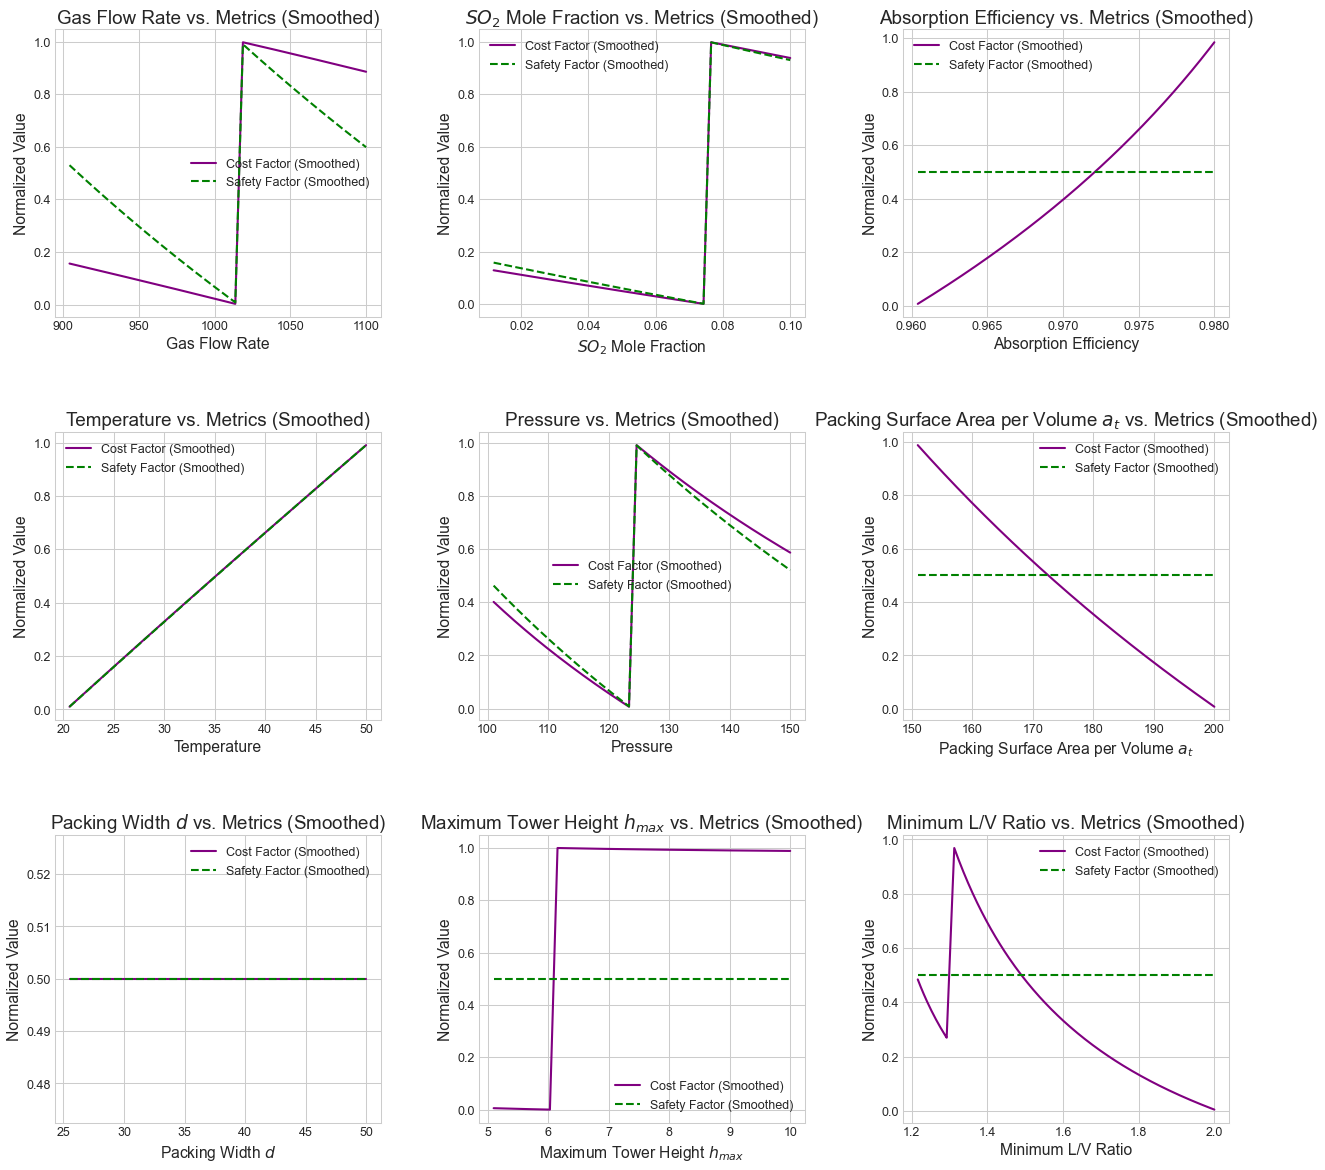
\includegraphics[width=0.8\textwidth]{trends.png}
	\caption{决策变量对成本因素和安全因素的影响趋势}
	\label{fig:trends}
\end{figure}

\clearpage

从图中可以观察到:

\begin{itemize}
	\item 气体流量的增加会导致成本因素和安全因素同时上升。
	\item 气相中二氧化硫含量的增加会导致成本因素下降,但安全因素也会降低。
	\item 二氧化硫吸收率的提高会增加成本因素,但同时也会提高安全因素。
\end{itemize}

这些趋势分析为我们后续的多目标优化提供了重要的参考。

\subsection{相关性分析方法}

为了确定哪些变量对成本因素和安全因素影响最大,我们进行了相关性分析。具体步骤如下:

\begin{enumerate}
	\item 对每个变量,在其可能的取值范围内取200个均匀分布的点。
	\item 固定其他变量,仅改变当前变量的值。
	\item 计算每个点对应的成本因素和安全因素。
	\item 使用Pearson相关系数计算变量与成本因素、安全因素的相关性。
\end{enumerate}

相关性系数的计算公式如下:

\begin{equation}
	r = \frac{\sum_{i=1}^{n} (x_i - \bar{x})(y_i - \bar{y})}{\sqrt{\sum_{i=1}^{n} (x_i - \bar{x})^2} \sqrt{\sum_{i=1}^{n} (y_i - \bar{y})^2}}
\end{equation}
其中,$x_i$和$y_i$分别表示变量和因素(成本或安全)的值,$\bar{x}$和$\bar{y}$表示它们的平均值。

\subsection{相关性分析结果}

通过相关性分析,我们得到了每个变量与成本因素和安全因素的相关系数。结果如表\ref{tab:correlation}所示。

\begin{table}[h]
	\centering
	\caption{变量与成本因素和安全因素的相关系数}
	\label{tab:correlation}
	\begin{tabular}{lcc}
		\hline
		变量 & 成本因素相关性 & 安全因素相关性 \\
		\hline
		气体流量 & 0.8036 & 0.5080 \\
		气相中二氧化硫含量 & 0.7276 & 0.7137 \\
		二氧化硫吸收率 & 0.9951 & -0.0000 \\
		操作温度 & 1.0000 & 1.0000 \\
		操作压力 & 0.6063 & 0.5222 \\
		填料总比表面积 & -0.9981 & 0.0000 \\
		填料直径 & nan & -0.0000 \\
		单个填料吸收塔最大高度 & -0.7055 & 0.0000 \\
		取最小液气比的比例常数 & -0.6191 & -0.0000 \\
		\hline
	\end{tabular}
\end{table}

根据相关性分析结果,可选择相关性最高的几个变量作为关键变量进行后续优化。

\section{多目标优化}

\subsection{基本假设}

\begin{enumerate}
	\item 吸收填料塔的成本因素仅与塔径和塔高有关。
	\item 填料的成本与填料塔的体积成正比。
	\item 不考虑塔内附件和塔外附件对成本、安全的影响,因填料塔工艺参数及填料确定内外附属部件可由此确定,所需成本也随即确定。
\end{enumerate}

\subsection{决策变量}
现对如下九个变量关于成本因素、安全因素进行相关性分析和趋势性分析。

\begin{enumerate}
	\item 气体流量,$V$
	\item 气相中二氧化硫含量,$Y_{1}$
	\item 二氧化硫吸收率,$\eta$
	\item 操作温度,$T$
	\item 操作压力,$P$
	\item 填料总比表面积,$a_{t}$
	\item 填料直径,$d$
	\item 单个填料吸收塔最大高度,$h_{max}$
	\item 取最小液气比的比例常数,$\big(\frac{L}{V}\big)_{min\,ratio}$
\end{enumerate}

\subsection{优化目标}

本章节优化目标为:
\begin{enumerate}
	\item 最小化吸收填料塔的成本因素,$Cost\,Factor$
	\item 最大化吸收填料塔的安全因素,$Safety\,Factor$
\end{enumerate}

这两个目标通常是相互矛盾的,因为提高安全性通常会增加成本。因此,我们需要在这两个目标之间寻找一个平衡点。

基于前面的分析,我们将吸收填料塔的优化问题定义为一个多目标优化问题:

\begin{equation}
	\begin{aligned}
		& \text{minimize}   & & f_1(\mathbf{x}) \quad \text{(成本因素)} \\
		& \text{maximize}   & & f_2(\mathbf{x}) \quad \text{(安全因素)} \\
		& \text{subject to} & & \mathbf{x}_l \leq \mathbf{x} \leq \mathbf{x}_u
	\end{aligned}
\end{equation}
其中,$\mathbf{x}$是决策变量向量,$\mathbf{x}_l$和$\mathbf{x}_u$分别是决策变量的下界和上界。

\subsection{NSGA-II算法}

为了解决这个多目标优化问题,我们选择使用NSGA-II(Non-dominated Sorting Genetic Algorithm II)算法。NSGA-II是一种高效的多目标优化算法,它具有以下特点:

\begin{itemize}
	\item 使用快速非支配排序方法
	\item 采用拥挤度距离来保持解的多样性
	\item 精英策略,确保最优解不会在进化过程中丢失
\end{itemize}

NSGA-II的主要步骤如下:

\begin{enumerate}
	\item 初始化种群
	\item 对种群进行非支配排序
	\item 计算拥挤度距离
	\item 选择、交叉和变异操作生成子代
	\item 合并父代和子代,进行精英选择
	\item 重复步骤2-5,直到达到终止条件
\end{enumerate}

\subsection{优化结果}

通过运行NSGA-II算法,我们得到了一系列非支配解,即帕累托前沿。图\ref{fig:pareto}展示了优化结果的帕累托前沿。

\begin{figure}[h]
	\centering
	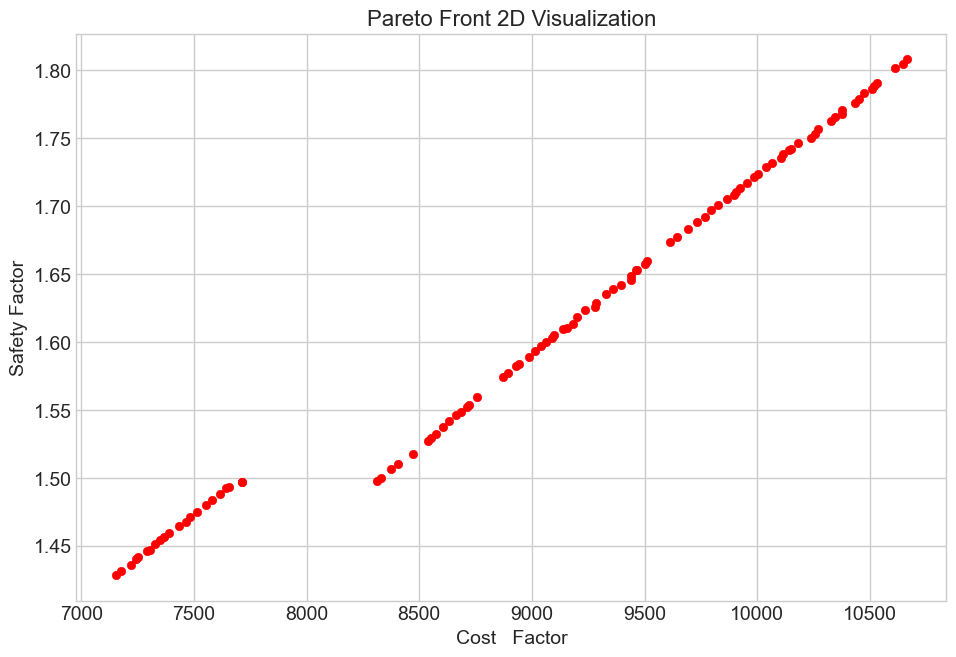
\includegraphics[width=\textwidth]{pareto_front.png}
	\caption{优化结果的帕累托前沿}
	\label{fig:pareto}
\end{figure}

从帕累托前沿可以看出,成本因素和安全因素之间存在明显的权衡关系。决策者可以根据具体需求,从帕累托前沿上选择合适的解。

表\ref{tab:optimal_solutions}列出了帕累托前沿上的一些代表性解。

\begin{table}[h]
	\footnotesize
	\centering
	\caption{帕累托前沿上的代表性解}
	\label{tab:optimal_solutions}
	\begin{tabular}{cccccccccc}
		\hline
		解 & 气体流量 & \ce{SO2}含量 & 吸收率 & 温度 & 压力 & 填料比表面积 & 填料宽度 & 最大塔高 & 最小$\big(\frac{L}{V}\big)$比率 \\
		\hline
		1 & 49.77 & 300.00 & 0.96 & 900.05 & 0.01 & 109.72 & 42.91 & 9.68 & 2.00 \\
		2 & 49.73 & 295.97 & 0.96 & 900.03 & 0.01 & 109.72 & 42.77 & 9.79 & 2.00 \\
		3 & 49.79 & 300.00 & 0.96 & 900.00 & 0.07 & 149.89 & 41.70 & 9.79 & 2.00 \\
		4 & 50.00 & 300.00 & 0.96 & 900.03 & 0.01 & 100.03 & 42.58 & 9.97 & 2.00 \\
		5 & 49.77 & 300.00 & 0.96 & 900.08 & 0.02 & 143.88 & 43.84 & 10.00 & 2.00 \\
		6 & 49.70 & 300.00 & 0.96 & 900.00 & 0.02 & 118.19 & 39.48 & 9.99 & 2.00 \\
		7 & 49.99 & 299.99 & 0.96 & 900.02 & 0.01 & 143.49 & 34.46 & 9.69 & 2.00 \\
		8 & 49.97 & 299.97 & 0.96 & 900.01 & 0.03 & 118.54 & 33.68 & 8.79 & 2.00 \\
		9 & 49.97 & 299.97 & 0.96 & 900.01 & 0.01 & 111.59 & 33.69 & 8.77 & 2.00 \\
		10 & 49.99 & 300.00 & 0.96 & 900.02 & 0.01 & 114.97 & 34.44 & 9.51 & 2.00 \\
		\hline
	\end{tabular}
\end{table}

\clearpage

\begin{table}[h]
	\small
	\centering
	\caption{优化结果的代表性目标值}
	\label{tab:objective_values}
	\begin{tabular}{c@{\hspace{0.35\textwidth}}r@{\hspace{0.3\textwidth}}c}
		\hline
		优化结果 & 成本因素 & 安全因素 \\
		\hline
		1 & 7107 & 1.43 \\
		2 & 10658 & 1.81 \\
		3 & 8255 & 1.50 \\
		4 & 7627 & 1.50 \\
		5 & 8786 & 1.57 \\
		6 & 10001 & 1.73 \\
		7 & 8851 & 1.58 \\
		8 & 9911 & 1.72 \\
		9 & 10459 & 1.79 \\
		10 & 10250 & 1.76 \\
		\hline
	\end{tabular}
\end{table}

通过对吸收填料塔的多目标优化研究,我们得出以下结论:

\begin{enumerate}
	\item 气体流量、\ce{SO2}含量和吸收率是影响成本因素和安全因素最显著的变量。
	\item 成本因素和安全因素之间存在明显的权衡关系,无法同时实现两者的最优。
	\item NSGA-II算法能够有效地找到吸收填料塔设计的帕累托最优解集。
\end{enumerate}

基于以上结论,我们提出以下建议:

\begin{enumerate}
	\item 在实际设计中,应根据具体需求在成本和安全之间寻找平衡点。
	\item 可以考虑使用本研究中的优化方法来辅助吸收填料塔的设计决策。
	\item 在条件允许的情况下,可以进一步考虑其他因素(如环境影响)进行多目标优化。
\end{enumerate}
	
	% 结论 or 总结	
	%%% 结论
\begin{conclusion}

本设计针对\ce{SO2}吸收填料塔进行了全面的工艺设计和计算,旨在实现高效的\ce{SO2}气体净化和分离。通过详细分析吸收剂的选择、吸收操作的流程、填料的类型和规格、以及塔内件的设计,我们确定了以20 $\circ C$清水作为吸收剂,采用逆流操作流程,并选择了DN25聚丙烯散装鲍尔环作为填料。在工艺设计中,我们计算了液相和气相的物性数据,进行了物料衡算,并确定了操作温度和压力。

在填料塔工艺尺寸的计算中,我们通过泛点率校核、填料规格校核和液体喷淋密度核算,确保了塔径和填料层高度的合理性。此外,我们还计算了传质单元数和传质单元高度,以确保填料塔的传质效率。最终,我们设计了一个直径为1000mm,填料层高度为5.7m的填料吸收塔,并计算了填料层的压降,确保了操作的经济性和安全性。

在塔内件的设计中,我们选择了槽式液体分布器、驼峰型支撑装置和抽屉式丝网除沫器,以保证气液的均匀分布和高效除沫。通过这些设计,我们预期能够实现\ce{SO2}吸收率大于等于98\%的分离要求,同时保证塔的稳定运行和高效传质。

综上所述,本设计不仅满足了\ce{SO2}吸收填料塔的基本工艺要求,而且在提高传质效率、降低能耗和维护成本方面做出了优化。通过本次设计,我们为化工、环保、石油和天然气处理等领域的气体净化和组分分离提供了一个高效、经济和可靠的解决方案。

\end{conclusion}
	
	% 参考文献
	% 注:至少引用一篇参考文献,否则执行全编译时下面两行会引起编译错误
	\nocite{*}
	\bibliographystyle{gbt7714-numerical}
	\bibliography{thesisbib.bib}
	
	% 符号说明
	%%% 符号说明
\begin{denotation}[11cm]\label{chap*:deno}%
	$M_V$              & 摩尔质量,g/mol                \\
	$\rho_V$           & 气体密度,kg/m³                \\
	$D_V$              & 气体扩散系数,m²/s             \\
	$\mu_V$            & 气体粘度,Pa·s                 \\
	$E$                & 亨利常数,kPa                  \\
	$m$                & 气体分子质量比,量纲一          \\
	$\rho_L$           & 液体密度,kg/m³                \\
	$\mu_L$            & 液体粘度,Pa·s                 \\
	$\sigma_L$         & 表面张力,N/m                  \\
	$D_L$              & 液体扩散系数,m²/s             \\
	$H$                & 溶解度系数,kmol/(kPa·m³)      \\
	$Y_1$              & 进料气体组分,量纲一            \\
	$Y_2$              & 出料气体组分,量纲一            \\
	$V$                & 气体流量,kmol/h               \\
	$\left(\frac{L}{V}\right)_{min}$  & 液气比,量纲一         \\
	$\left(\frac{L}{V}\right)_{min\_ratio}$  & 最小液气比,量纲一 \\
	$\frac{L}{V}$      & 实际液气比,量纲一              \\
	$L$                & 液体流量,kmol/h               \\
	$X_1$              & 进料液体组分,量纲一            \\
	$W_L$              & 液体质量流量,kg/h              \\
	$W_V$              & 气体质量流量,kg/h              \\
	$X_{Eckert, \phi_F}$ & 泛点气速Eckert坐标X值,量纲一  \\
	$Y_{Eckert, \phi_F}$ & 泛点气速Eckert坐标Y值,量纲一  \\
	$u_F$              & 泛点气速,m/s                  \\
	$u_{design}$       & 设计气速,m/s                  \\
	$D$                & 未圆整塔径,m                  \\
	$D_{rounded}$      & 圆整后塔径,量纲一              \\
	$u_{actual}$       & 实际操作气速,m/s              \\
	$flooding \, ratio$ & 泛点率,量纲一                 \\
	$\frac{D_{rounded}}{d}$ & 圆整后塔径与填料直径比,量纲一 \\
	$U_{min}$          & 最小喷淋密度,m³/(m²·h)        \\
	$U$                & 实际喷淋密度,m³/(m²·h)        \\
	$S$                & 脱吸因数,m²                   \\
	$N_{OG}$           & 气相总传质单元数,量纲一         \\
	$U_L$              & 液相质量通量,kg/(m²·h)        \\
	$\frac{a_w}{a_t}$  & 有效比表面积比,量纲一           \\
	$a_w$              & 有效比表面积,m²/m³            \\
	$U_V$              & 气相质量通量,kg/(m²·h)        \\
	$k_G$              & 气膜吸收系数,kmol/(m²·h·kPa)  \\
	$k_L$              & 液膜吸收系数,m/h              \\
	$k_{G}a$           & 气膜体积吸收系数,kmol/(m²·h·kPa) \\
	$k_{L}a$           & 液膜体积吸收系数,m/h          \\
	$k'_{G}a$          & 修正后的气膜体积吸收系数,kmol/(m²·h·kPa) \\
	$k'_{L}a$          & 修正后的液膜体积吸收系数,m/h  \\
	$K_{G}a$           & 总传质系数,kmol/(m²·h·kPa)    \\
	$H_{OG}$           & 填料层高度,m                  \\
	$Z$                & 总高度,m                      \\
	$Z'$               & 设计高度,m                    \\
	$X_{Eckert, \phi_P}$ & 填料层压降Eckert坐标X值,量纲一 \\
	$Y_{Eckert, \phi_P}$ & 填料层压降Eckert坐标Y值,量纲一 \\*
\end{denotation}

	
	% 附录
	\appendix
	%%% 附录A
\chapter{工艺参数处理代码}



%%% ===============================================
\section{计算工艺参数}
\lstinputlisting[
	language=python,
	caption=吸收填料塔工艺参数处理代码,
	label=code:absorabsorption_column
	]{code/absorption_column.py}

\section{定义优化问题}	
\lstinputlisting[
	language=python,
	caption=吸收塔问题类定义了三个优目标:经济最低,安全最大,符合最大,
	label=code:absorption_problem
	]{code/absorption_problem.py}

\section{选择关键变量}
\lstinputlisting[
	language=python,
	caption=控制变量分析,敏感度分析,相关性分析,
	label=code:variables_analysis
	]{code/variables_analysis.py}

\section{实现目标优化}
\lstinputlisting[
	language=python,
	caption=提取关键变量用遗传算法,梯度下降实现最优化,
	label=code:multiobjective_optimize
	]{code/multiobjective_optimize.py}
	%%% 设计图纸
\chapter{设计图纸}



%%% ===============================================
\begin{dfigure}[H]
	\centering
	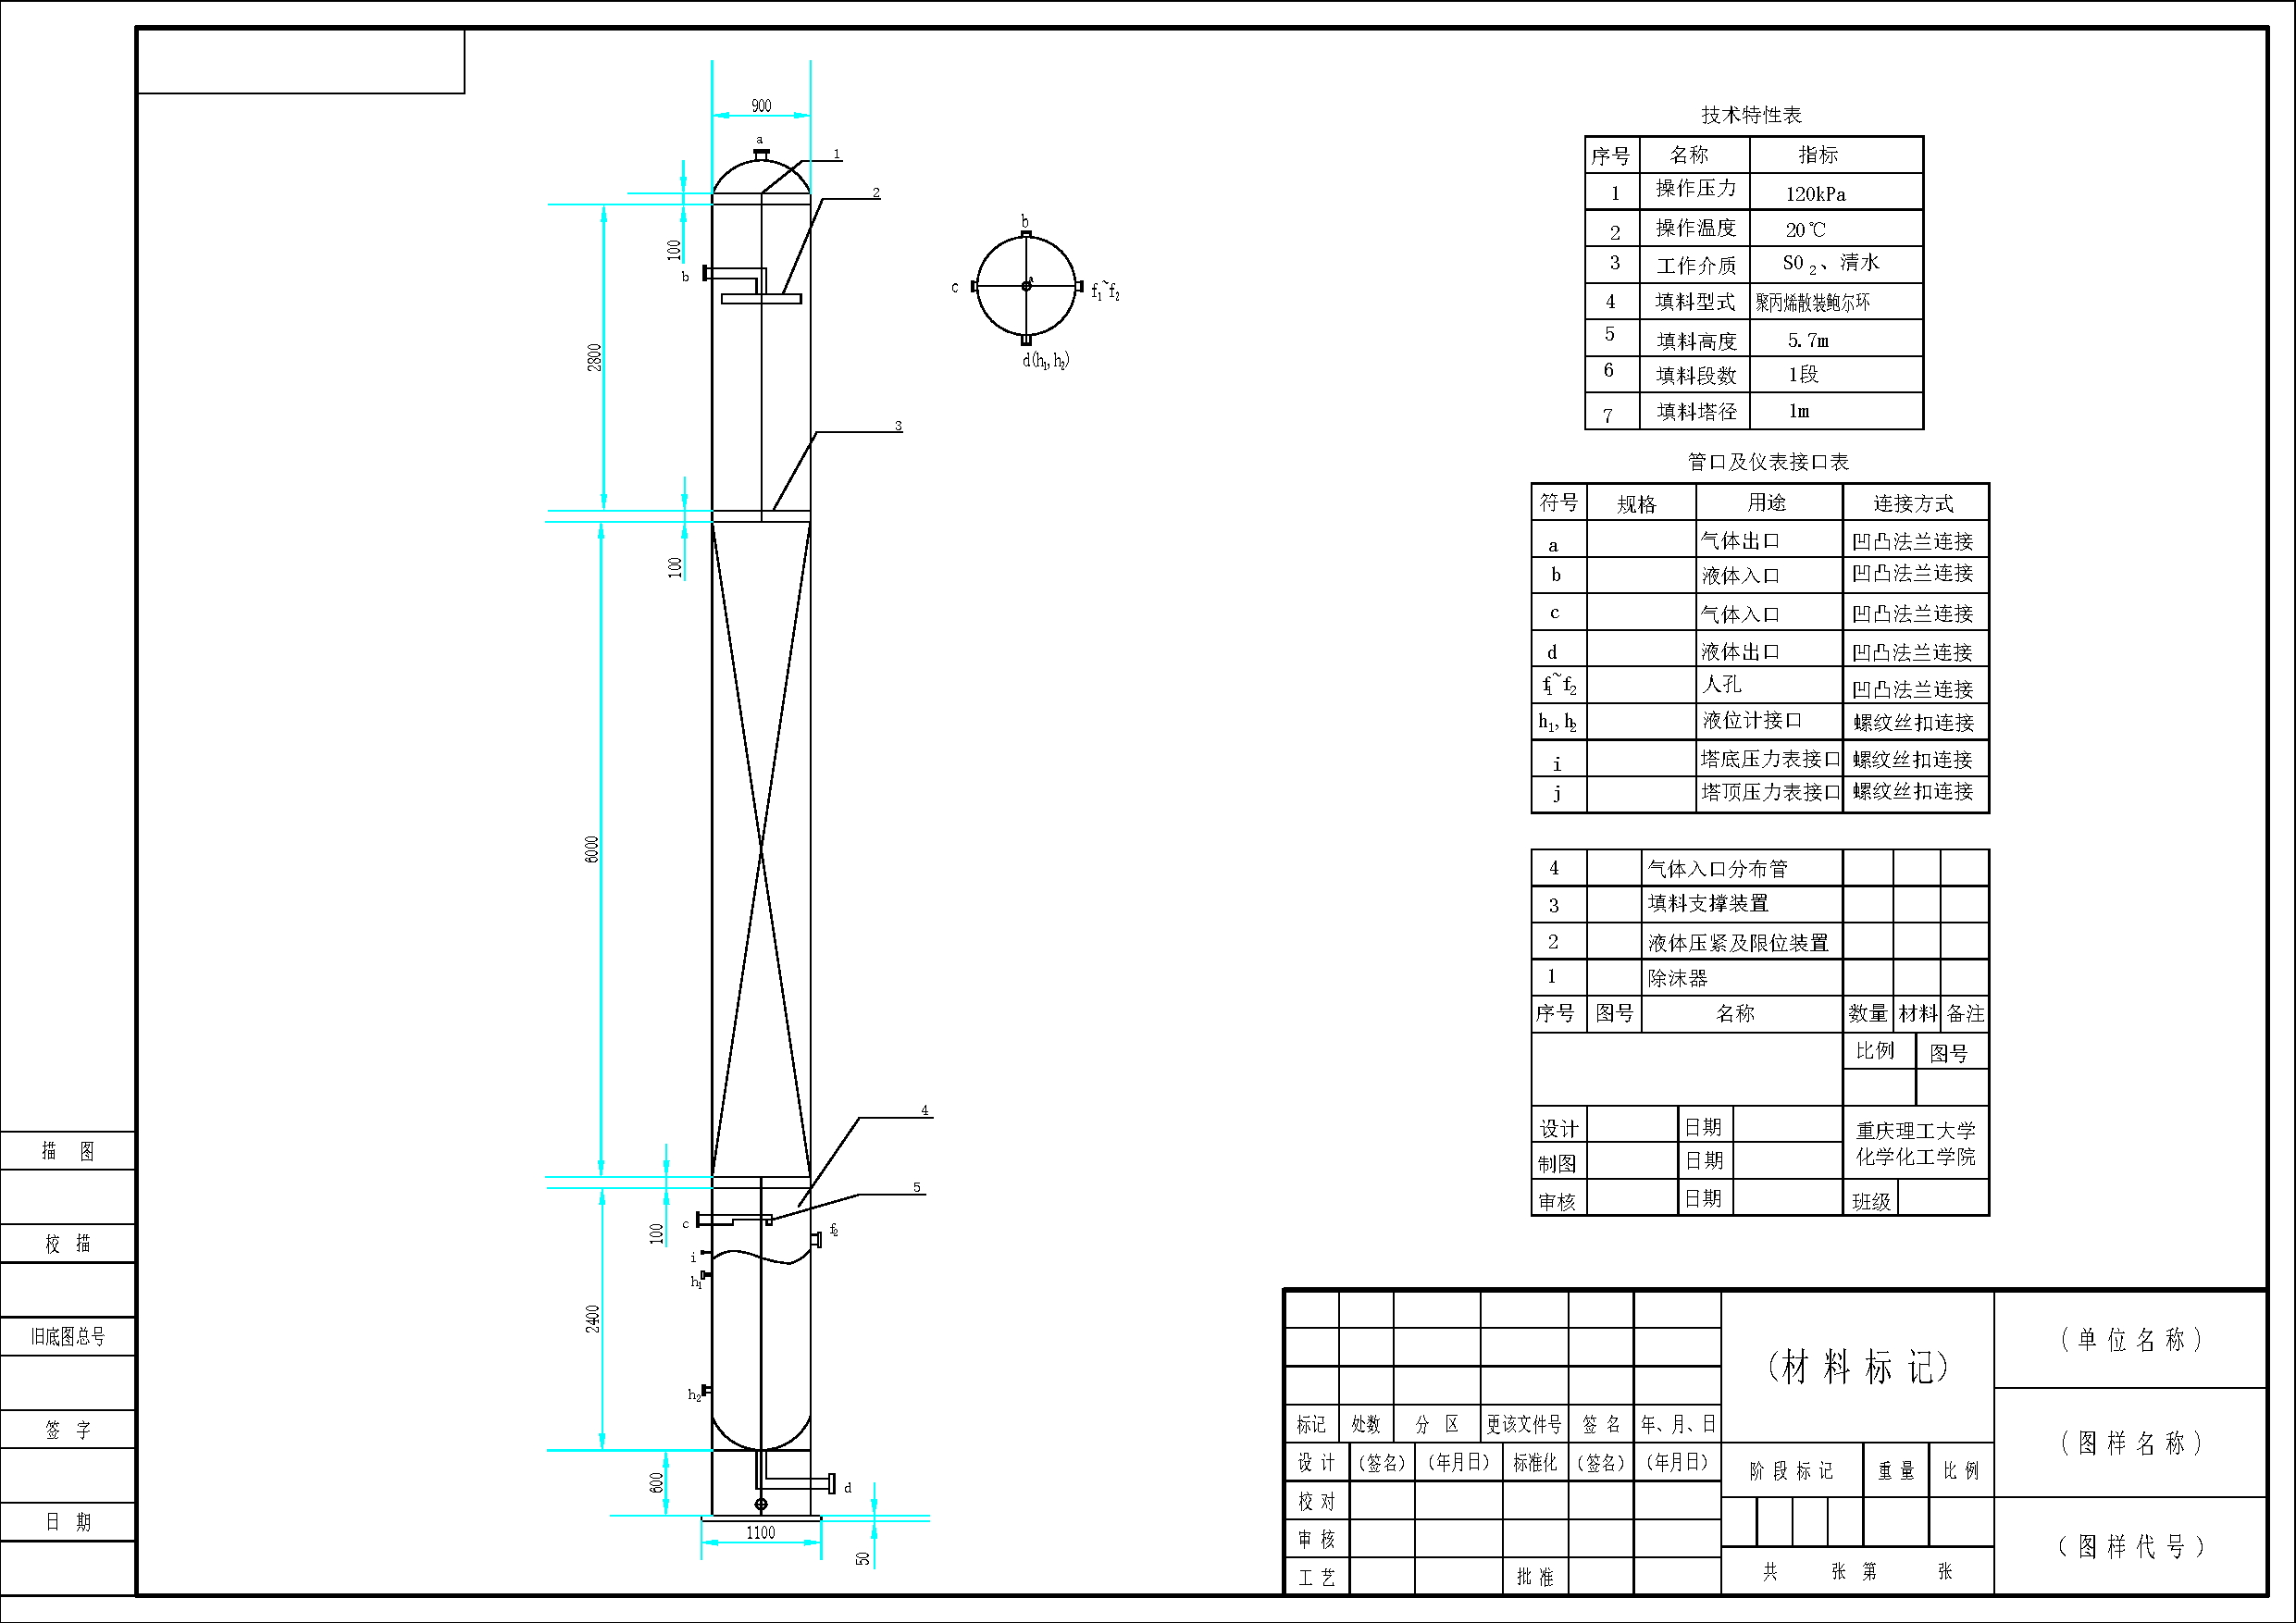
\includegraphics[width=1.25\textwidth, angle=-90]{吸收填料塔工艺参数条件-模型.pdf}
	\dcaption{SO2吸收填料塔工艺参数条件图} % 将设计图纸名称编入主目录
	\label{design:1}
\end{dfigure}

%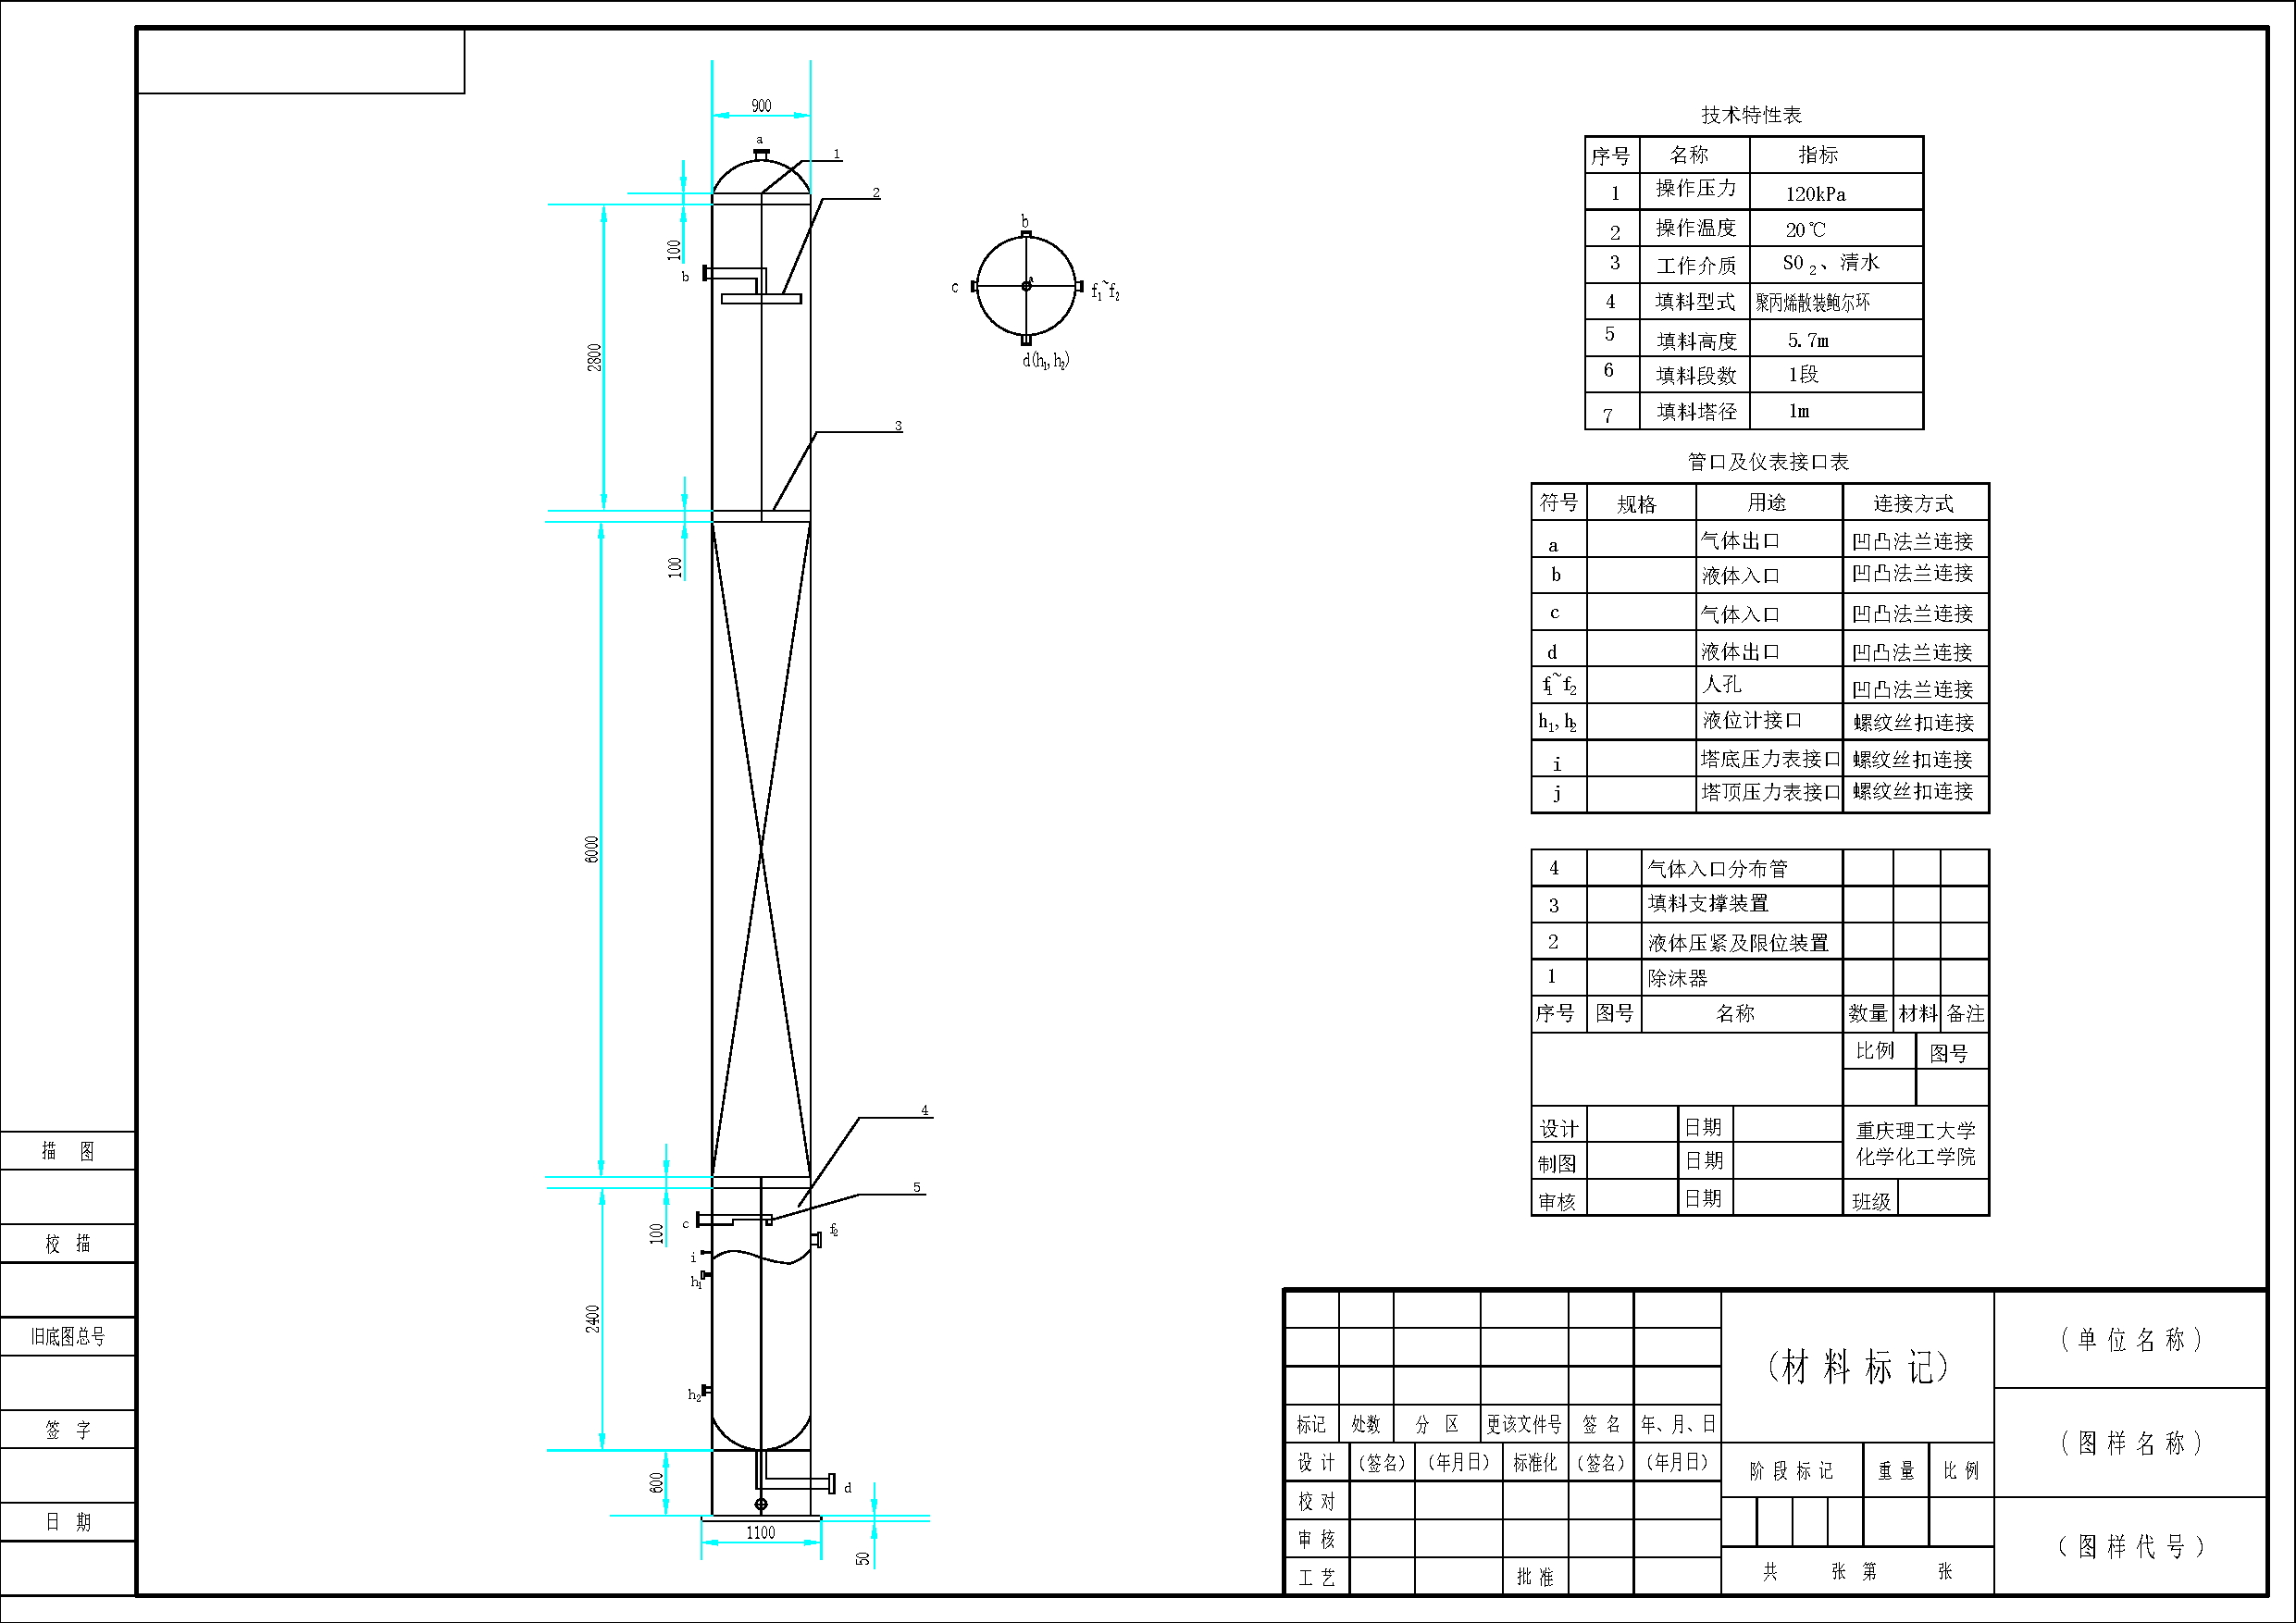
\includepdf[pages=-, angle=-90]{吸收填料塔工艺参数条件-模型.pdf}



\cleardoublepage
%%% ===============================================
\begin{dfigure}[H]
	\centering
	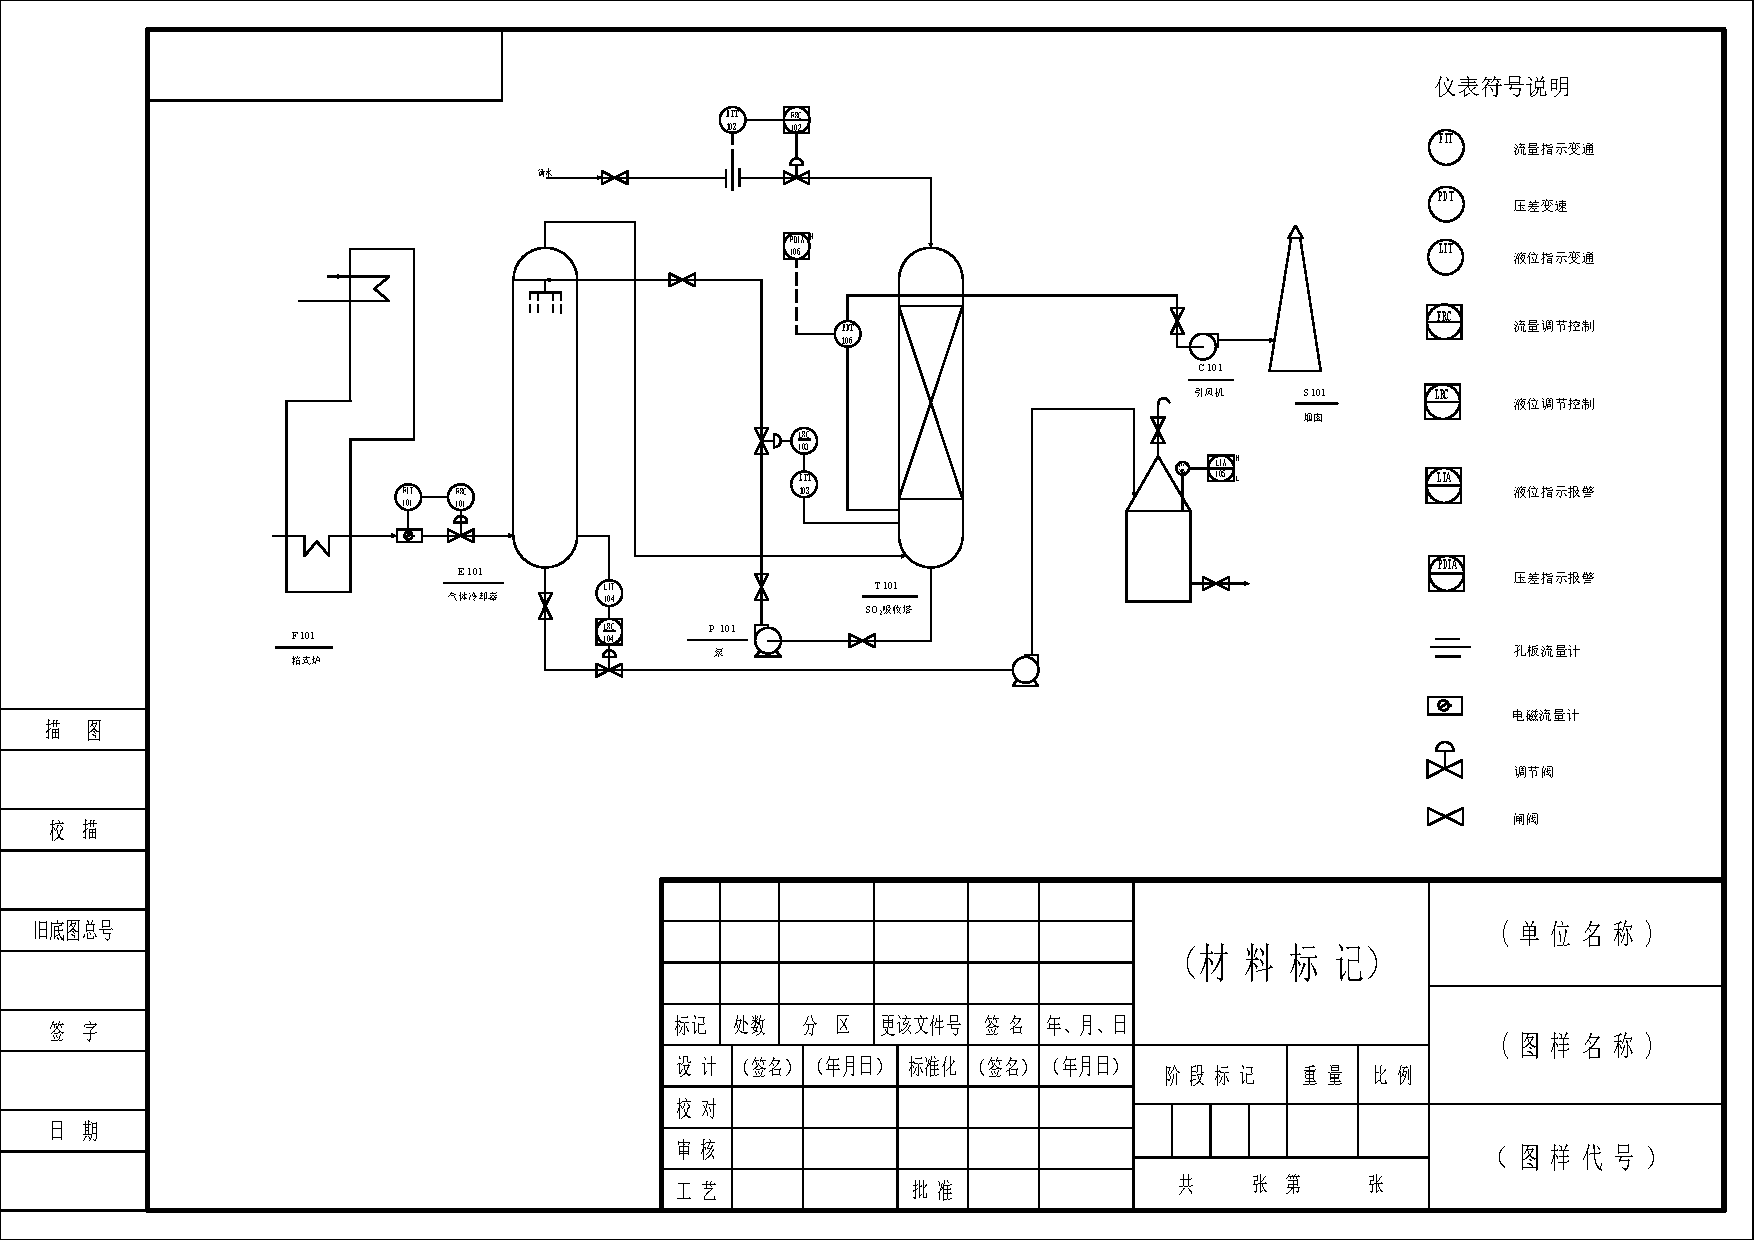
\includegraphics[width=1.25\textwidth,angle=-90]{SO2吸收工艺流程图-模型.pdf}
	\dcaption{SO2吸收工艺流程图} % 将设计图纸名称编入主目录
	\label{design:2}
\end{dfigure}

%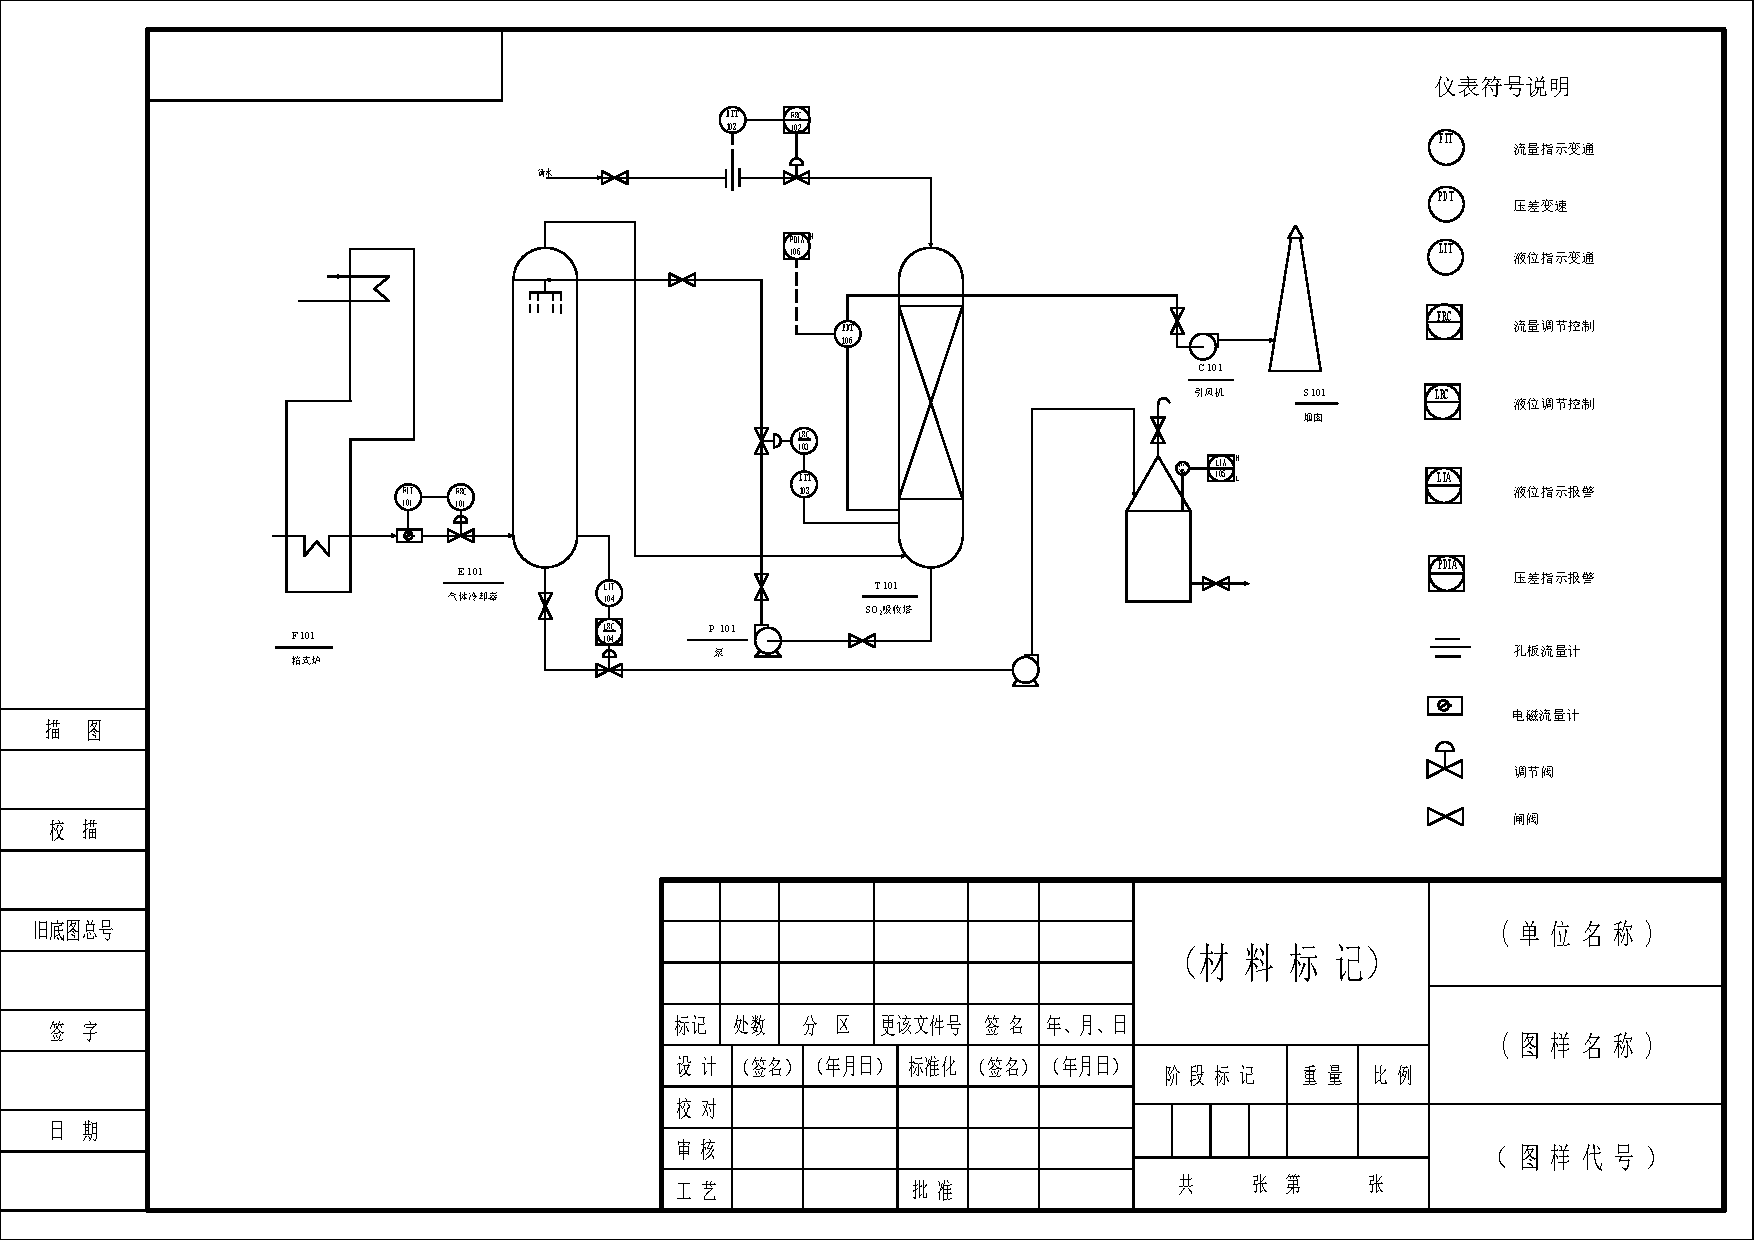
\includepdf[pages=-, angle=-90]{SO2吸收工艺流程图-模型.pdf}
	
\end{document}